%
% Template for OPTCON course projects
%
\documentclass[a4paper,11pt,oneside]{book}

\usepackage{titlesec}

\titleformat{\chapter}[display]
  {\normalfont\bfseries}{}{0pt}{\Huge}
  
\usepackage[latin1]{inputenc}
\usepackage[english]{babel}
\usepackage{amsfonts}
\usepackage{amsmath}
\usepackage{amssymb,amsmath,color}
\usepackage{cite}
\usepackage{graphicx}
\usepackage{float}

\begin{document}
\pagestyle{myheadings}

%%%%%%%%%%% Cover %%%%%%%%%%%
\thispagestyle{empty}                                                 
\begin{center}                                                            
    \vspace{5mm}
    {\LARGE UNIVERSIT\`A DI BOLOGNA} \\                       
      \vspace{5mm}
\end{center}
\begin{center}
  
\includegraphics[scale=.27]{pictures/logo_unibo}
\end{center}
\begin{center}
      \vspace{5mm}
      {\LARGE School of Engineering} \\
        \vspace{3mm}
      {\Large Master Degree in Automation Engineering} \\
      \vspace{20mm}
      {\LARGE Optimal Control} \\

      \vspace{5mm}{\Large\textbf{Course Project $-$ Group 5\\Optimal Control of a Quadrotor with Suspended Load}}                  
      \vspace{15mm}
\end{center}
\begin{flushleft}                                                                              
     {\large Professor: \textbf{\@ Giuseppe Notarstefano}} \\        
      \vspace{13mm}
\end{flushleft}
\begin{flushright}
      {\large Students:} Friz Anna\\
      Ruscelli Gabriele\\
      Valeri Eleonora
\end{flushright}        %capoverso allineato a destra
\begin{center}
\vfill
      {\large Academic year \@2023/2024} \\
\end{center}



\newpage
\thispagestyle{empty}

%%%%%%%%%%% Abstract %%%%%%%%%%%%
\begin{center}
\chapter*{}
\thispagestyle{empty}
{\Huge \textbf{Abstract}}\\
\vspace{15mm}

This project addresses the optimal control of a planar quadrotor with a suspended load. Tasks involve dynamics discretization, trajectory generation through the Newton's method algorithm, trajectory tracking via Linear Quadratic Regulator (LQR) and Model Predictive Control (MPC).
Finally, the quadrotor movement will be shown in an animation.
\end{center}

\tableofcontents \thispagestyle{empty}
% \listoffigures\thispagestyle{empty}

%%%%%%%%%% Introduction %%%%%%%%%%
\chapter*{Introduction}
\addcontentsline{toc}{chapter}{Introduction}

In this project, we are required to design an optimal trajectory for a quadrotor with a suspended load. 

The project consists of four main steps:
\begin{itemize}
  \item Task 0 - Problem Setup:
Discretization of the quadrotor dynamics and writing of the iscrete-time state-space equations.
  \item Task 1 - Trajectory Generation I:
Design of an optimal trajectory to move from one equilibrium configuration to another, using a Newton's like algorithm.
  \item Task 2 - Trajectory Generation II:
Generation of a desired (smooth) state$-$input curve and
application of the trajectory generation task (Task 1) on this new desired trajectory.
    \item Task 3 - Trajectory Tracking via LQR:
Linearization of the model around the optimal trajectory obtained in the previous point and definition of the optimal feedback controller to perform trajectory tracking through LQR algorithm.
    \item Task 4 - Trajectory
tracking via MPC: Exploitation of an MPC algorithm to track the optimal trajectory $(x_{opt}, u_{opt})$ computed in Task 2 linearizing the vehicle dynamics about it.
    \item Task 5 - Animation:
Producing a simple animation of the vehicle executing Task 3.
\end{itemize}



%%%%%%%%%% Chapters %%%%%%%%%

\chapter{Task 0 - Problem setup}
In task 0 we want to discretize the dynamics, write the discrete-time state-space equations and code the
dynamics function.

\section{State space and control inputs}
The system can be modeled as a planar quadrotor with a downward pendulum attached
at its center of mass, representing the load,
as shown in Figure \ref{fig:quadrotor}.

\begin{figure}[htp]
\centering
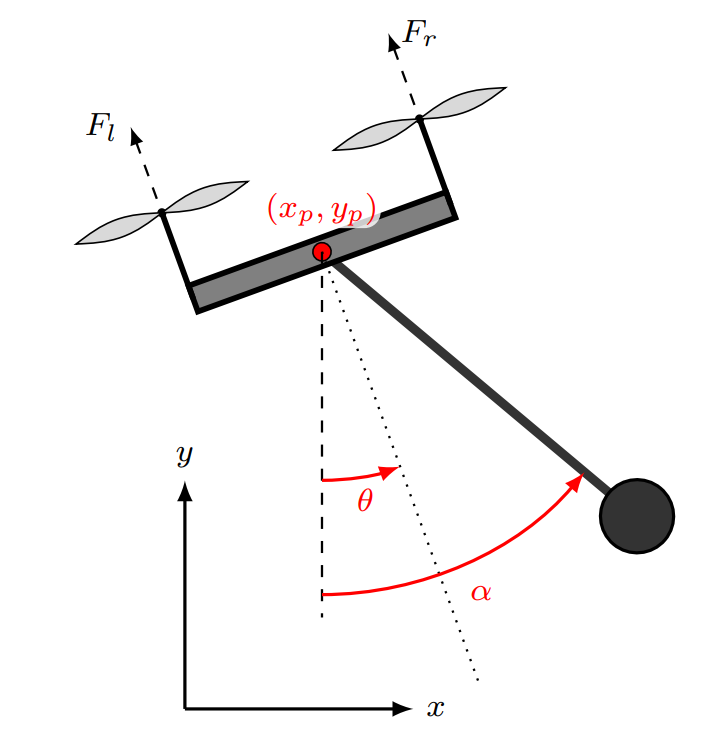
\includegraphics[width=0.5\textwidth]{pictures/quadrotor}
\caption{Model of a planar quadrotor with a suspended load}
\label{fig:quadrotor}
\end{figure}

The state space consist in \[ x = [x_p, y_p, \alpha, \theta, v_x, v_y, \omega_\alpha, \omega_\theta]^T\] where $(x_p, y_p) \in \mathbb{R}^2$ represent the position of the center of mass, $\theta$ the roll angle of the quadrotor, $\alpha$ the angle of the pendulum with respect to the inertial frame, $(v_x, v_y)$ the velocity of the center of mass, $\omega_\alpha$ and $\omega_\theta$ angular rate of changes associated to $\alpha$ and $\theta$, respectively.

The input is \[u = [F_s, F_d]^T\] where \[\begin{cases}F_s = F_l + F_r \\ F_d = F_r - F_l\end{cases}\] and $(F_l, F_r)$ are the forces generated by the propellers.
\\



The dynamical model is described by:
\[
\begin{cases}
(M+m) \dot{v}_x  = m L \omega_\alpha^2 sin(\alpha) - F_s (sin(\theta) - \frac{m}{M} sin(\alpha - \theta) cos(\alpha))\\
(M+m) \dot{v}_y  = - m L \omega_\alpha^2 cos(\alpha) + F_s (cos(\theta) + \frac{m}{M} sin(\alpha - \theta) sin(\alpha)) - \frac{m}{M} g\\
M L \dot{\omega}_\alpha = - F_s sin(\alpha - \theta)\\
J \dot{\omega}_\theta = l F_d\\
\end{cases}
\]

Where, all the parameters of the quadrotor are: 

\begin{center}
\begin{tabular}{ |c|c|c| } 
 \hline
 M: mass of the drone & 0.028 [kg] \\ 
 m: mass of the load & 0.04 [kg] \\ 
 J: inertia of the drone & 0.001 $[kg m^2]$\\ 
 g: gravity & 9.81 $[m/s^2]$\\ 
 L: length of the pendulum & 0.2 [m]\\ 
 l: distance from center of mass to propeller & 0.5 [m]\\ 
 \hline
\end{tabular}
\end{center}


\section{Forward Euler discretization}
In order to write the discrete-time state-space equations, we consider the discrete time version of the drone dynamics, discretized via forward Euler: 
\[
x_{t+1}  = x_t + \delta f_{CT} (x_t, u_t, t)\\
\]

where $\delta > 0$ is a sufficiently small discretization step and $\delta f_{CT} (., ., .)$ is the continuous-time dynamics. In particular, we choose $\delta = 1e^{-2}$. 


We obtain the following discrete-time state-space equations: 
\[
\begin{cases}
x_{1,t+1} = x_{1,t} + \delta x_{5,t} \\
x_{2,t+1} = x_{2,t} + \delta x_{6,t} \\
x_{3,t+1} = x_{3,t} + \delta x_{7,t} \\
x_{4,t+1} = x_{4,t} + \delta x_{8,t} \\
x_{5,t+1} = x_{5,t} + \frac{\delta}{m+M} [m L x_{7,t}^2 sin(x_{3,t}) - u_{1,t} (sin(x_{4,0}) + \\ \qquad \qquad \qquad - \frac{m}{M} sin(x_{3,t} - x_{4,t}) cos(x_{3,t}))]  \\
x_{6,t+1} = x_{6,t} + \frac{\delta}{m+M} [(-m L x_{7,t}^2 cos(x_{3,t}) + u_{1,t} (cos(x_{4,0}) + \\
\qquad \qquad \qquad +\frac{m}{M} sin(x_{3,t} - x_{4,t}) sin(x_{3,t})))-g] \\
x_{7,t+1} = x_{7,t} + \frac{\delta}{M L} [-u_{1,t} sin(x_{3,t} - x_{4,t})] \\
x_{8,t+1} = x_{8,t} + \frac{\delta}{J} l u_{2,t}
\end{cases} 
\]

In which state and input vectors are: 
\[ \textbf{x}_t = \begin{bmatrix} x_{p,t} \\ y_{p,t} \\ \alpha_t \\ \theta_t \\ v_{x,t} \\ v_{y,t} \\ \omega_{\alpha,t} \\ \omega_{\theta,t} \end{bmatrix} = \begin{bmatrix}   x_{1,t} \\ x_{2,t} \\ x_{3,t} \\ x_{4,t} \\ x_{5,t} \\ x_{6,t} \\ x_{7,t} \\ x_{8,t} \end{bmatrix} \]

\[ \textbf{u}_t = \begin{bmatrix} F_{s,t} \\ F_{d,t} \end{bmatrix} = \begin{bmatrix}   u_{1,t} \\ u_{2,t} \end{bmatrix} \]



\section{Jacobians computation}
For future purposes the gradient with respect to state and input are calculated.
\[
\textbf{A}
=
\begin{bmatrix}
    1 & 0 & 0 & 0 & 0 & 0 & 0 & 0 \\
    0 & 1 & 0 & 0 & 0 & 0 & 0 & 0 \\
    0 & 0 & 1 & 0 & a_{3,5} & a_{3,6} & a_{3,7} & 0 \\
    0 & 0 & 0 & 1 & a_{4,5} & a_{4,6} & a_{4,7} & 0 \\
    \delta  & 0  & 0 & 0 & 1 & 0 & 0 & 0 \\
    0 & \delta & 0 & 0 & 0 & 1 & 0 & 0 \\
    0 & 0 & \delta & 0 & a_{7,5} & a_{7,6} & 1 & 0 \\
    0 & 0 & 0 & \delta & 0 & 0 & 0 & 1 
\end{bmatrix}
\]

with 
\[a_{3,5} = \frac{\delta}{m+M} (m L x_{7,t}^2 cos(x_{3,t}) + u_{1,t} \frac{m}{M} cos(2 x_{3,t} - x_{4,t})) \]
\[a_{4,5} = \frac{\delta u_{1,t}}{m+M} (cos(x_{4,t}) + \frac{m}{M} cos(x_{3,t} - x_{4,t}) cos(x_{3,t}))\]
\[a_{7,5} = \frac{2 \delta}{m+M} m L x_{7,t} sin(x_{3,t})\]
\[a_{3,6} = \frac{\delta u_{1,t} m}{m+M} (cos(x_{3,t}-x_{4,t}) sin(x_{4,t}) + sin(x_{3,t}-x_{4,t}) cos(x_{4,t}))\]
\[a_{4,6} = \frac{\delta}{m+M} (m L x_{7,t}^2 sin(x_{4,t}) - u_{1,t} sin(x_{4,t}) + \frac{m}{M} cos(x_{3,t}-x_{4,t}) sin(x_{3,t}))\]
\[a_{7,6} = \frac{-2\delta}{m+M} (m L cos(x_{4,t}) x_{7,t}))\]
\[a_{3,7} = \frac{\delta}{ML} (-u_{1,t} cos(x_{3,t}-x_{4,t}))\]
\[a_{4,7} = \frac{\delta}{ML} (u_{1,t} cos(x_{3,t}-x_{4,t}))\]

and 

\[
\textbf{B}^T
=
\begin{bmatrix}
    0 & 0 & 0 & 0 & b_{1,5} & b_{1,6} & b_{1,7} & 0 \\
    0 & 0 & 0 & 0 & 0 & 0 & 0 & \delta l /J 
\end{bmatrix}
\]

with 
\[b_{1,5} = - \delta (sin(x_{4,t}) - \frac{m}{M} sin(x_{3,t} - x_{4,t}) cos(x_{3,t}))\]
\[b_{1,6} = \delta (cos(x_{4,t}) + \frac{m}{M} sin(x_{3,t}-x{4,t}) sin(x_{4,t}))\]
\[b_{1,7} = \frac{-\delta}{ML} sin(x_{3,t}-x_{4,t})\]

\section{\textit{Dynamics} function}
We can now code a dynamics function that takes as inputs $x_t\in \mathbb{R}^8, u_t\in \mathbb{R}^2$ and returns as output the next state $x_{t+1}\in \mathbb{R}^8$ and the gradient of the dynamics $\textbf{A}\in \mathbb{R}^{8x8}, \textbf{B}^T\in \mathbb{R}^{2x8}$

\begin{figure}[htp]
\centering
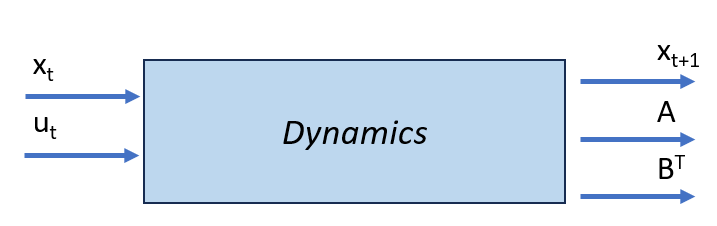
\includegraphics[width=0.5\textwidth]{pictures/dynamics.png}
\caption{\textit{Dynamics} function scheme block}
\label{fig:dynamics}
\end{figure}

\chapter{Task 1 - Trajectory generation (I)}
In task 1 we want to compute two equilibria for our system, define a reference curve between them and then compute the optimal transition to move from one equilibrium to another exploiting the Newton's$-$like algorithm for optimal control.

\section{Equilibrium Computation}

To compute the equilibria of the system, we set the derivatives of the system to zero:


\[
\begin{cases}
\begin{aligned}
&x_{5,t+1} - x_{5,t} = \frac{\delta}{m+M} \bigl[m L x_{7,t}^2 \sin(x_{3,t}) +\\
&\qquad - u_{1,t} \bigl(\sin(x_{4,0}) - \frac{m}{M} \sin(x_{3,t} - x_{4,t}) \cos(x_{3,t})\bigr)\bigr] = 0 \\
&x_{6,t+1} - x_{6,t} = \frac{\delta}{m+M} \bigl[(-m L x_{7,t}^2 \cos(x_{3,t}) +\\
&\qquad + u_{1,t} \bigl(\cos(x_{4,0}) + \frac{m}{M} \sin(x_{3,t} - x_{4,t}) \sin(x_{3,t})\bigr)\bigr) - g] = 0 \\
&x_{7,t+1} - x_{7,t} = \frac{\delta}{M L} [-u_{1,t} \sin(x_{3,t} - x_{4,t})] = 0 \\
&x_{8,t+1} - x_{8,t} = \frac{\delta}{J} l u_{2,t} = 0
\end{aligned}
\end{cases}
\]



Solving this system could lead to four possible configurations, but we will only consider the following case:
\[
\begin{cases}
x_{3,t} = 0\\
x_{4,t} = x_{3,t}\\
u_{1,t} = (M + m) g\\
u_{2,t} = 0
\end{cases}
\]

Note that this equilibrium point can represent either a stationary position or a constant velocity.

\section{Reference trajectory definition}

The planned path is made using the starting and ending equilibrium points. This path looks the same on both sides, with two long steady parts in between. Keep in mind that this reference trajectory is not a feasible trajectory for the system dynamics.

Here an example of reference trajectory.

\begin{figure}[h]
  \centering
  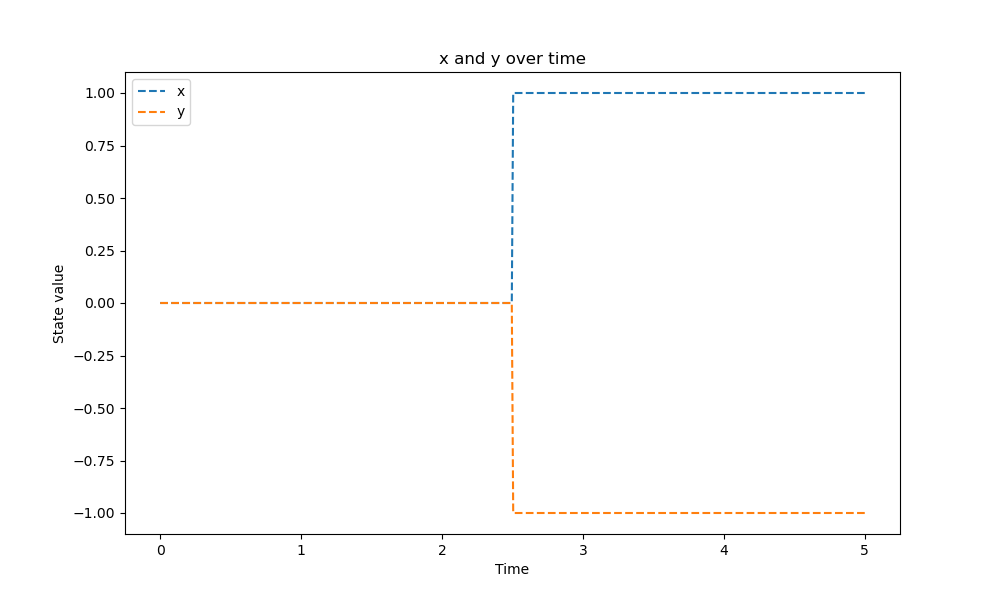
\includegraphics[width=0.9\textwidth]{pictures/x_y ref.png}\hfill\\
  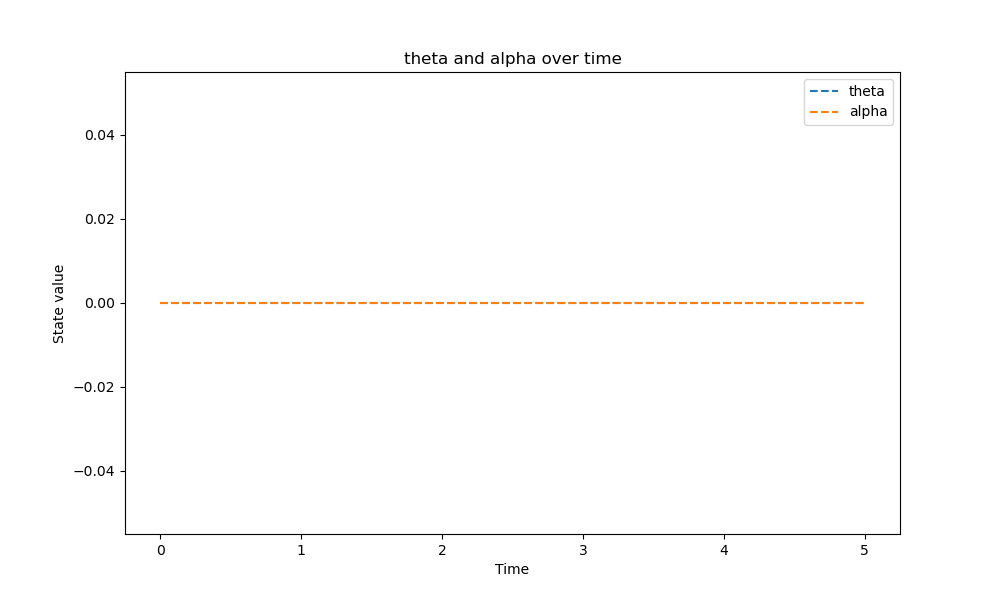
\includegraphics[width=0.9\textwidth]{pictures/theta_alpha ref.png}\hfill
  \caption{configuration reference over time.}
  \label{fig:Reference trajectory}
\end{figure}

\begin{figure}[H]
  \centering
  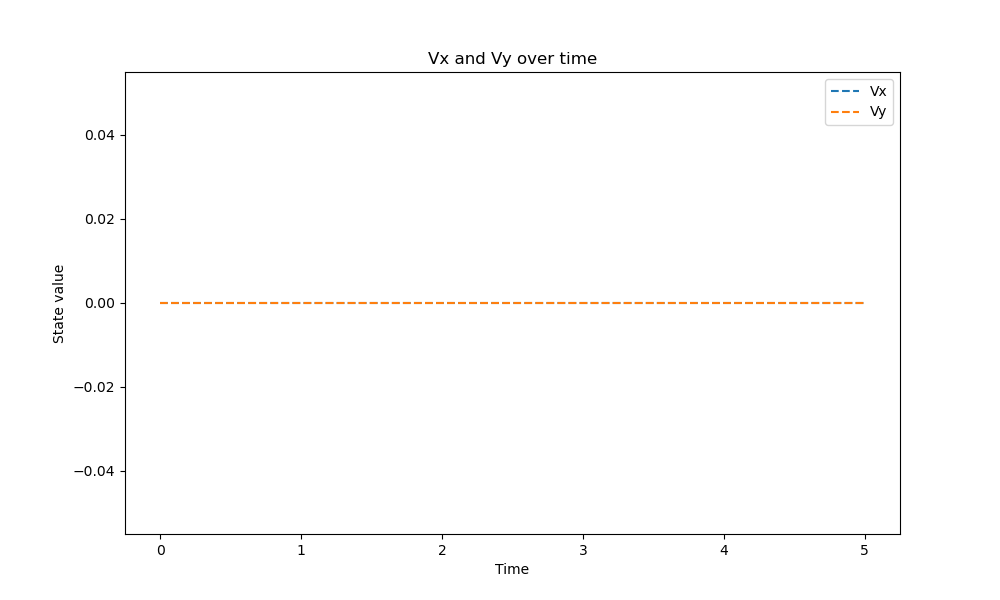
\includegraphics[width=0.85\textwidth]{pictures/Vx_vyreef.png}\hfill \\
  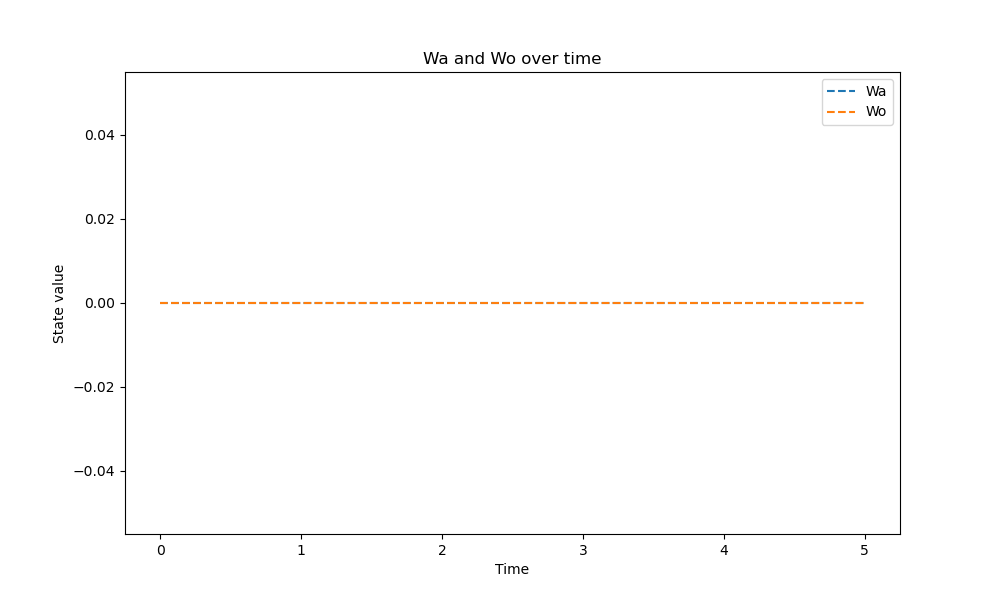
\includegraphics[width=0.85\textwidth]{pictures/wa wo ref.png}\hfill
  \caption{velocities reference over time.}
  \label{fig:Reference trajectory}
  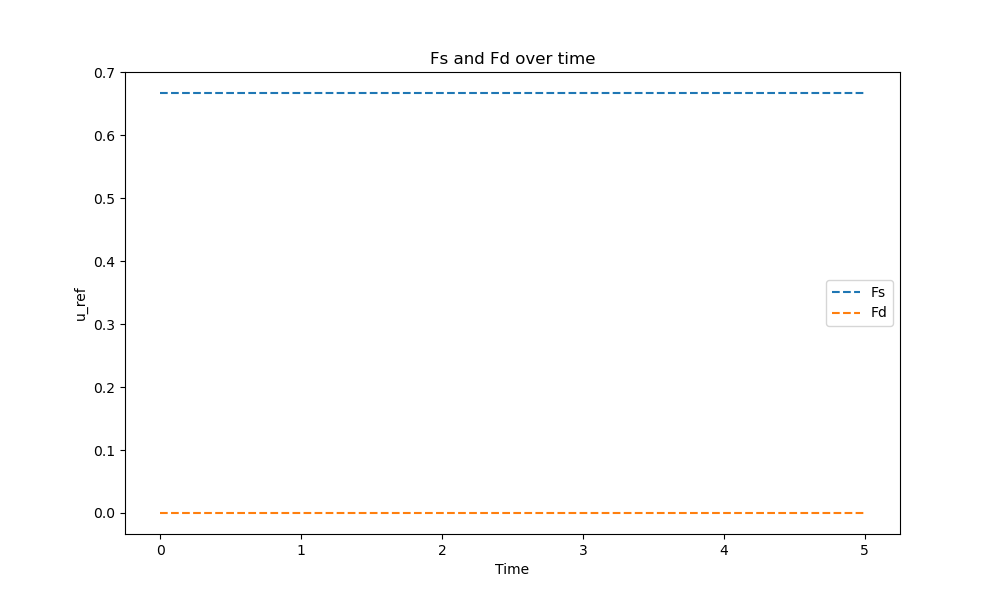
\includegraphics[width=0.85\textwidth]{pictures/Fs fd ref.png}
  \caption{Input reference over time.}
  \label{fig:Reference trajectory}
\end{figure}


\section{Linear Quadratic Regularization}
To solve the optimal control problem we implemented Linear Quadratic Regularization (LQR).
\subsection{Sketch of the algorithm}
\textbf{Initialization}\vspace{8pt}

Consider as initial guess trajectory the first equilibrium point $(x_0, u_0)$.

For $k = 0, 1, \ldots$:\vspace{8pt}

\textbf{Step 1: Compute Descent Direction}\vspace{8pt} \\
Linearize the system dynamics evaluating 
\[\nabla_1 f_t(x_k^t, u_k^t), \nabla_2 f_t(x_k^t, u_k^t), \nabla_1 \ell_t(x_k^t, u_k^t), \nabla_2 \ell_t(x_k^t, u_k^t), \nabla \ell_T(x_k^T)\] 
Compute the gradient of the reduced cost solving backwards the co-state equation, with $\lambda_k^T = \nabla \ell_T(x_k^T)$, and compute $Q_k^t$, $R_k^t$, $S_k^t$, and $Q_k^T$. \vspace{8pt}\\
In order to define the LQR controller compute $K_k^t$, $\sigma_k^t$, for all $t = 0, \ldots, T - 1$:
\begin{align*}
\min_{\Delta x, \Delta u} &\sum_{t=0}^{T-1} \left( \nabla_1 \ell_t(x_k^t, u_k^t) \Delta x_t + \nabla_2 \ell_t(x_k^t, u_k^t) \Delta u_t \right)^\top \begin{bmatrix} \Delta x_t \\ \Delta u_t \end{bmatrix} \\
&+ \frac{1}{2} \begin{bmatrix} \Delta x_t \\ \Delta u_t \end{bmatrix}^\top \begin{bmatrix} Q_k^t & S_k^{t,\top} \\ S_k^t & R_k^t \end{bmatrix} \begin{bmatrix} \Delta x_t \\ \Delta u_t \end{bmatrix} \\
&+ \nabla \ell_T(x_k^T)^\top \Delta x_T + \frac{1}{2} \Delta x_T^\top Q_k^T \Delta x_T
\end{align*}
\textbf{Step 2: Compute new state-input trajectory}\vspace{8pt} \\
Implementing step-size selection rule, e.g., Armijo) \\
Forward integrate (closed-loop), for all  t = 0, \ldots, T - 1,  with  $x_{k+1,0} = x_{\text{init}}$ \vspace{8pt}\\
$u_{k+1,t} = u_k^t + K_k^t (x_{k+1,t} - x_k^t)$

\subsection{Costs definition}
Two types of costs are used: in the case of position control, we give more weight to the position of the quadrotor, while in the case of velocity control, we give more weight to the cost of the quadrotor's velocity. \vspace{8pt}

Costs for Position Control:
\[
QQt = \begin{bmatrix}
10 & 0 & 0 & 0 & 0 & 0 & 0 & 0 \\
0 & 10 & 0 & 0 & 0 & 0 & 0 & 0 \\
0 & 0 & 1 & 0 & 0 & 0 & 0 & 0 \\
0 & 0 & 0 & 1 & 0 & 0 & 0 & 0 \\
0 & 0 & 0 & 0 & 1 & 0 & 0 & 0 \\
0 & 0 & 0 & 0 & 0 & 1 & 0 & 0 \\
0 & 0 & 0 & 0 & 0 & 0 & 1 & 0 \\
0 & 0 & 0 & 0 & 0 & 0 & 0 & 1 \\
\end{bmatrix}
\]
\[
RRt = \begin{bmatrix}
3 & 0 \\
0 & 3 \\
\end{bmatrix}
\]
\vspace{8pt}
\[
QQT = QQt
\]

Costs for Velocity Control:
\[
QQt_{\text{vel}} = \begin{bmatrix}
0.0001 & 0 & 0 & 0 & 0 & 0 & 0 & 0 \\
0 & 0.0001 & 0 & 0 & 0 & 0 & 0 & 0 \\
0 & 0 & 0.1 & 0 & 0 & 0 & 0 & 0 \\
0 & 0 & 0 & 0.1 & 0 & 0 & 0 & 0 \\
0 & 0 & 0 & 0 & 10 & 0 & 0 & 0 \\
0 & 0 & 0 & 0 & 0 & 10 & 0 & 0 \\
0 & 0 & 0 & 0 & 0 & 0 & 2 & 0 \\
0 & 0 & 0 & 0 & 0 & 0 & 0 & 2 \\
\end{bmatrix}
\]
\vspace{8pt}
\[
RRt_{\text{vel}} = \begin{bmatrix}
0.05 & 0 \\
0 & 0.05 \\
\end{bmatrix}
\]
\vspace{8pt}
\[
QQT_{\text{vel}} = QQt_{\text{vel}}
\]

\section{Results}
In this section, we present the outcomes of the Linear Quadratic Regulator on the previous example of reference trajectory.
\subsection{Optimal trajectory}
In the following pages the optimal trajectory found by our algorithm is shown.

\begin{figure}[H]
  \centering
  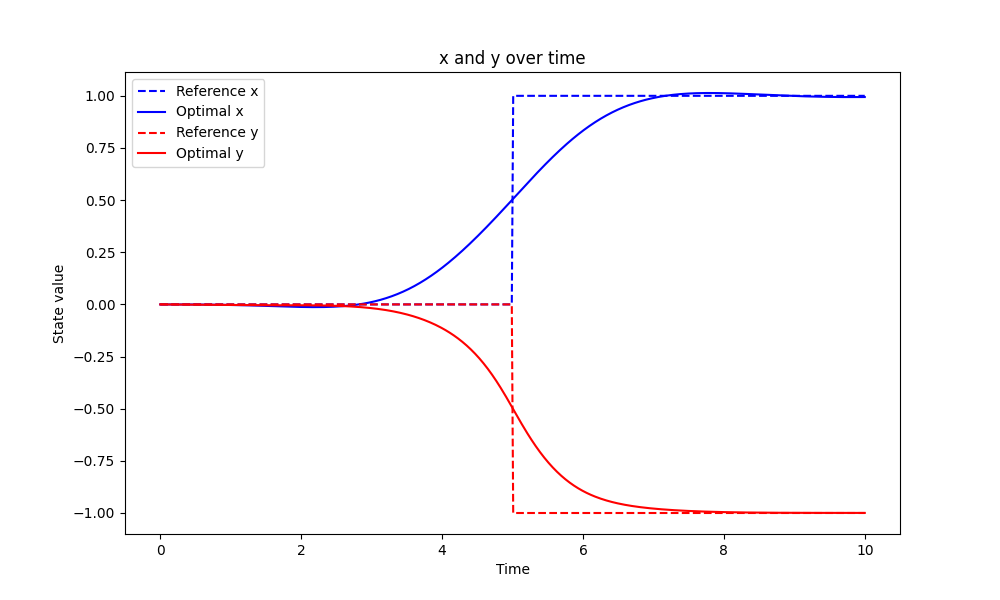
\includegraphics[width=1\textwidth]{pictures/x_y opt.png}\hfill \\
  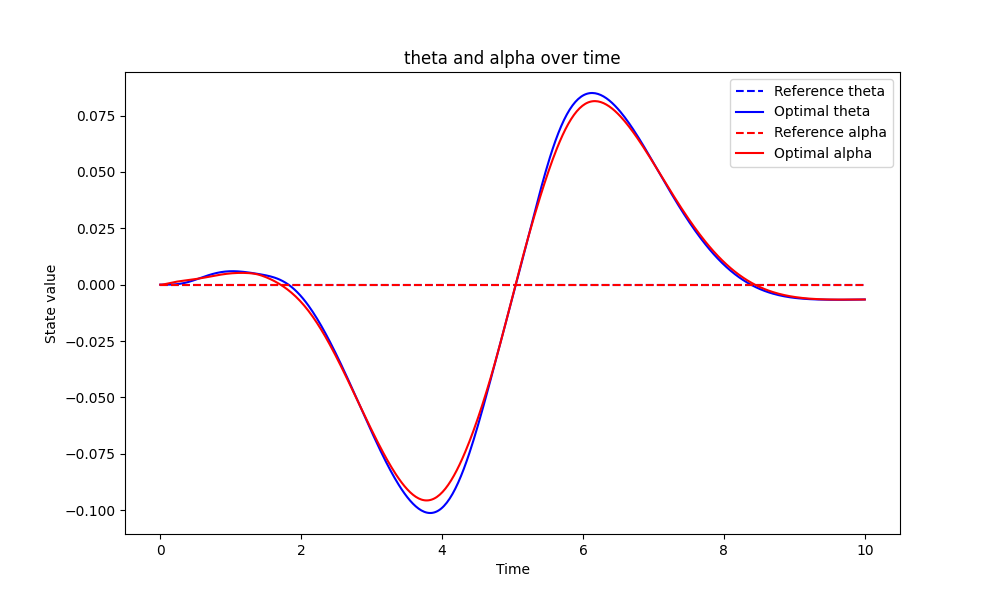
\includegraphics[width=1\textwidth]{pictures/theta alpha opt.png}\hfill
  \caption{Optimal configuration over time.}
  \label{fig:Reference trajectory}
\end{figure}

\begin{figure}[H]
  \centering
  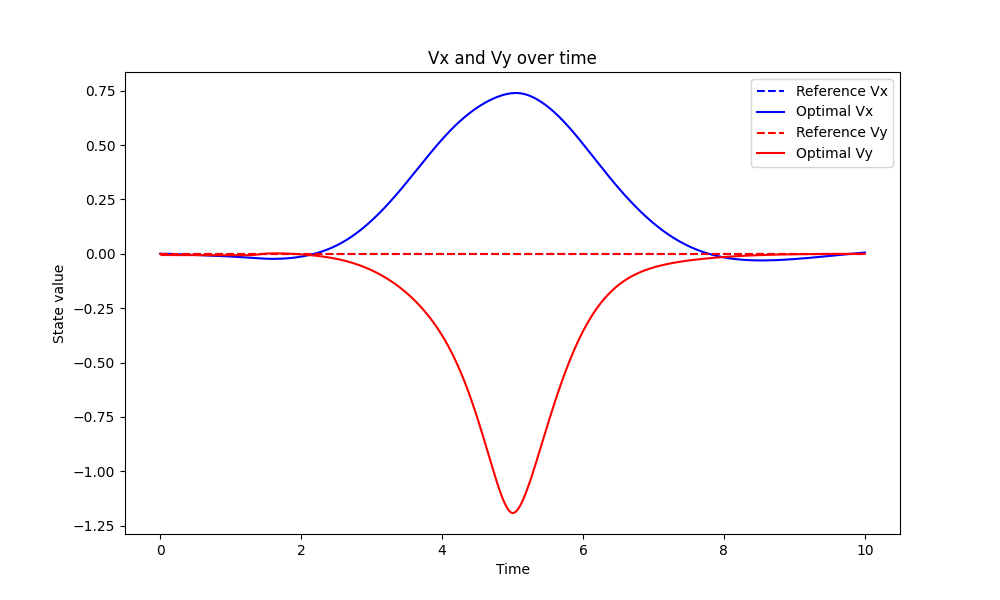
\includegraphics[width=0.85\textwidth]{pictures/vx and vy opt.png}\hfill \\
  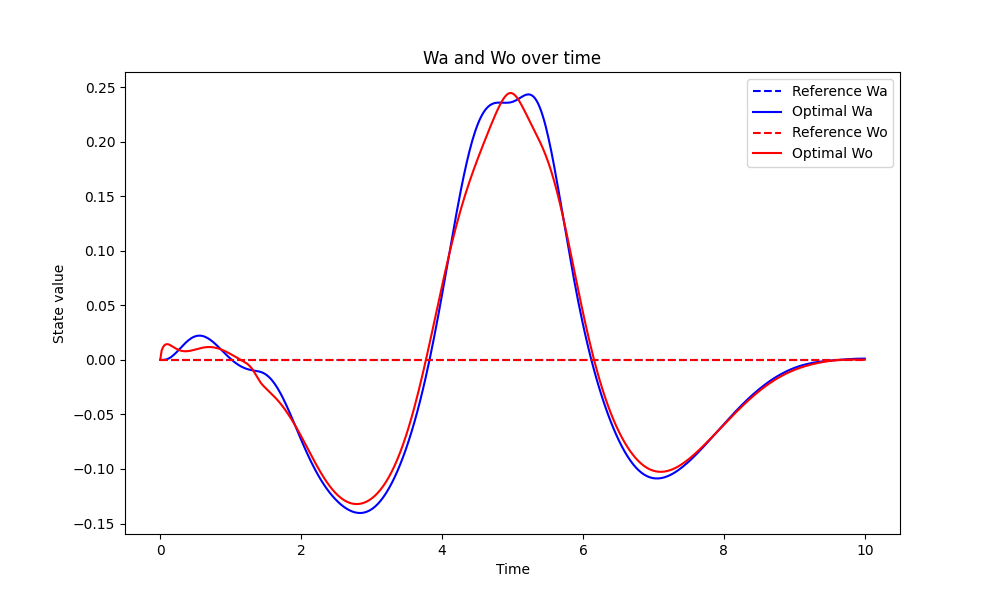
\includegraphics[width=0.85\textwidth]{pictures/omega alpha and theta.png}\hfill
  \caption{optimal velocities over time.}
  \label{fig:Reference trajectory}
  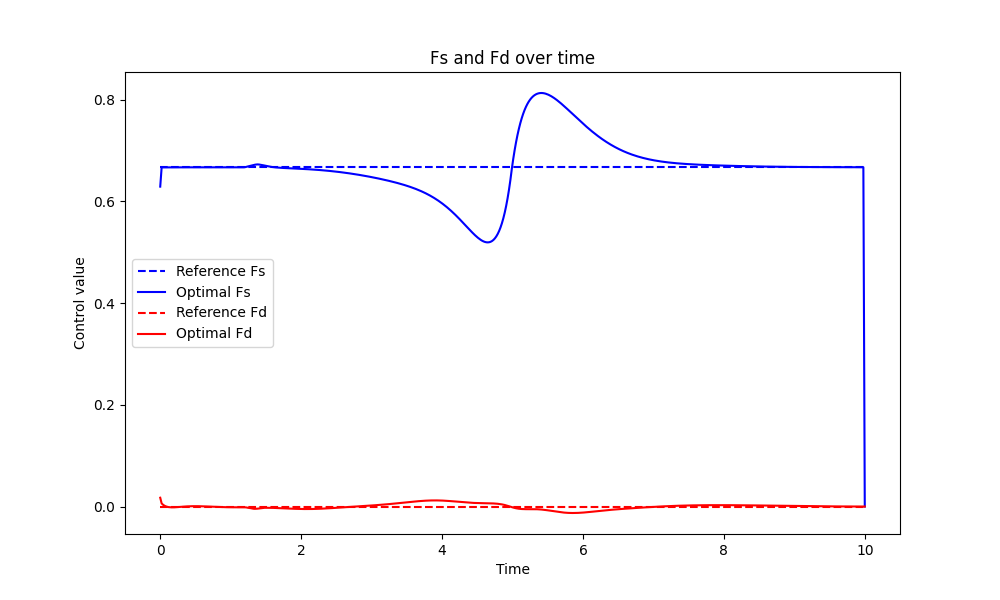
\includegraphics[width=0.85\textwidth]{pictures/Fs and Fd opt.png}
  \caption{Optimal input over time.}
  \label{fig:Reference trajectory}
\end{figure}



\subsection{Suboptimal trajectories}
To illustrate the iterative evolution of the algorithm, we display only the x and y coordinates of the quadrotor over time and the armijos plot, providing an overview of the overall progression. Refer to the code for more details.
\begin{figure}[H]
  \centering
  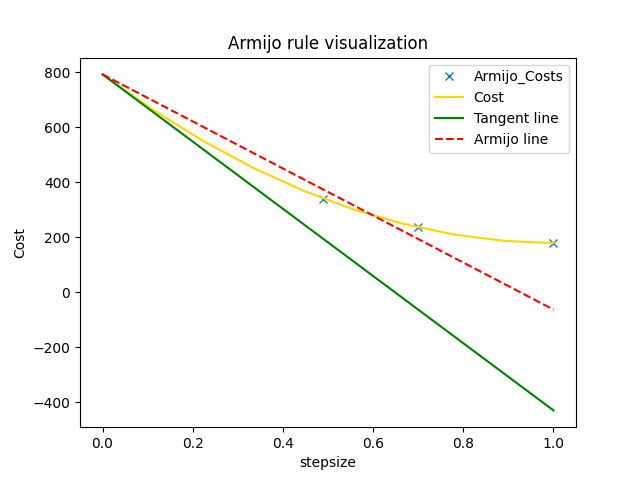
\includegraphics[width=1\textwidth]{pictures/arm_it_1.png}\hfill \\
  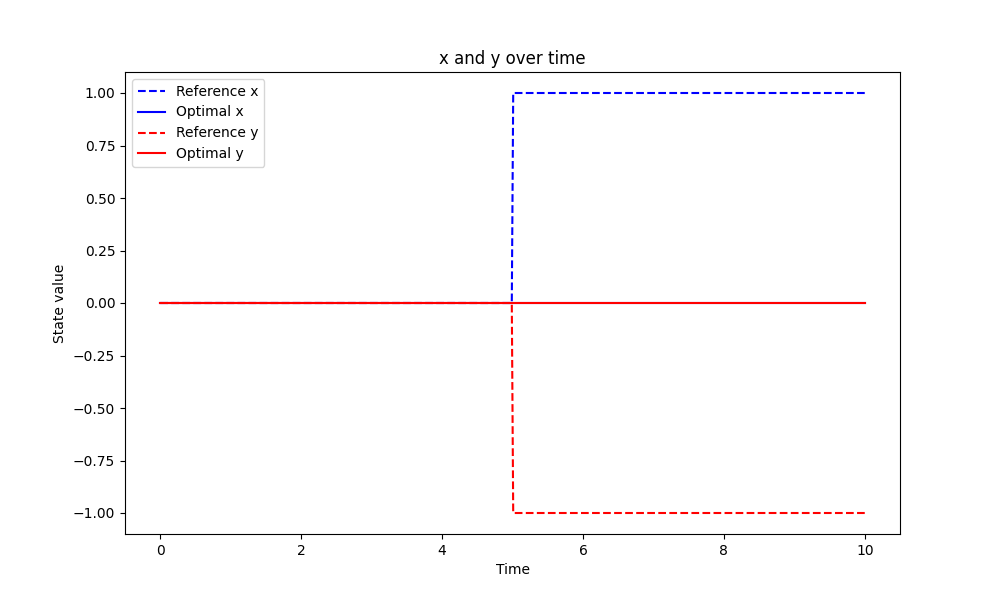
\includegraphics[width=1\textwidth]{pictures/new_it_1.png}\hfill
  \caption{First iteration.}
  \label{fig:Reference trajectory}
\end{figure}

\begin{figure}[H]
  \centering
  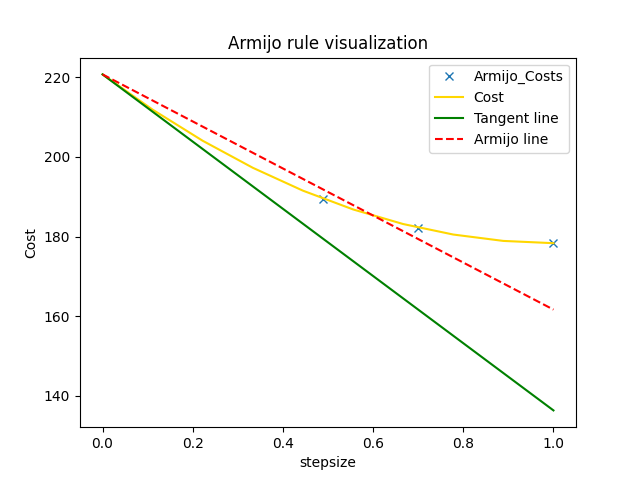
\includegraphics[width=1\textwidth]{pictures/arm_it_3.png}\hfill \\
  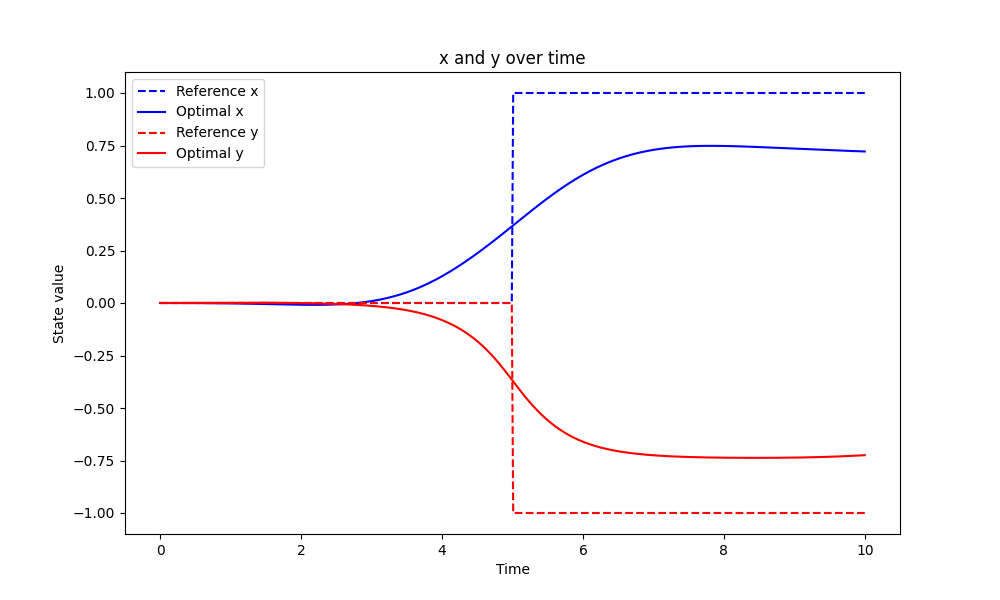
\includegraphics[width=1\textwidth]{pictures/new_it_3.png}\hfill
  \caption{Third iteration.}
  \label{fig:Reference trajectory}
\end{figure}

\begin{figure}[H]
  \centering
  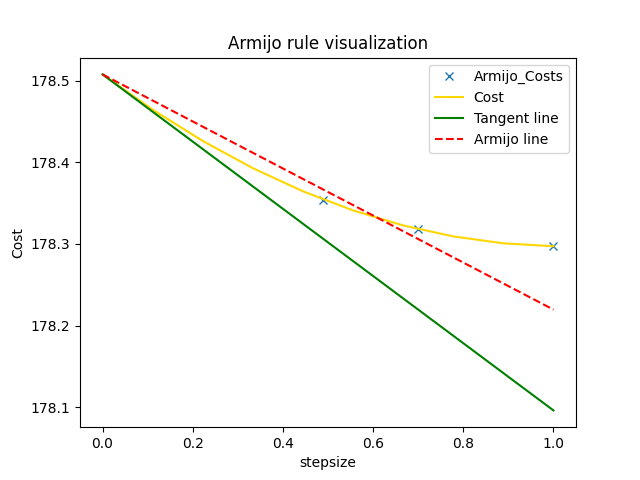
\includegraphics[width=1\textwidth]{pictures/arm_it_7.png}\hfill\\
  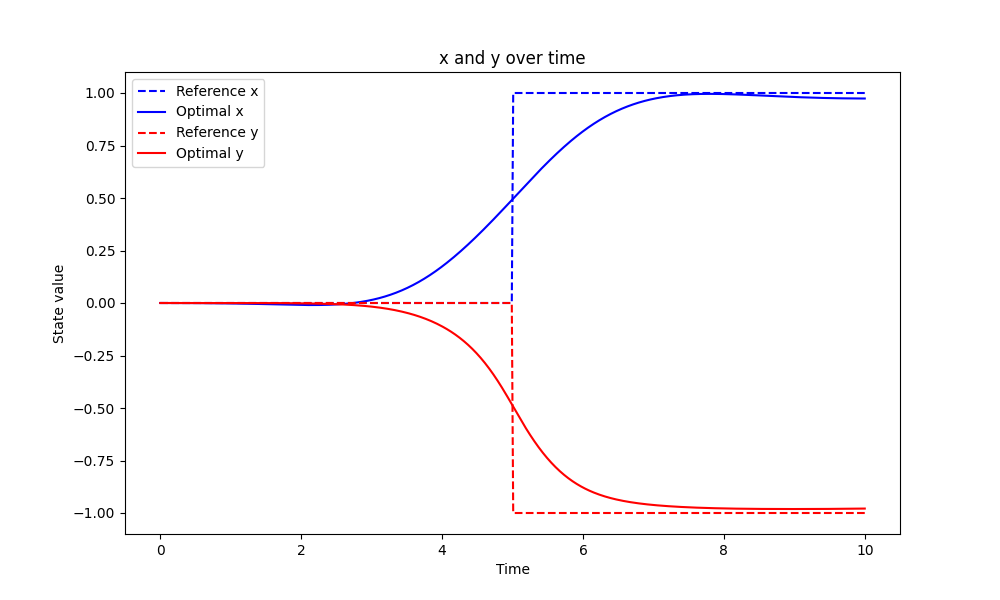
\includegraphics[width=1\textwidth]{pictures/new_it_7.png}\hfill
  \caption{Seventh iteration.}
  \label{fig:Reference trajectory}
\end{figure}

\begin{figure}[H]
  \centering
  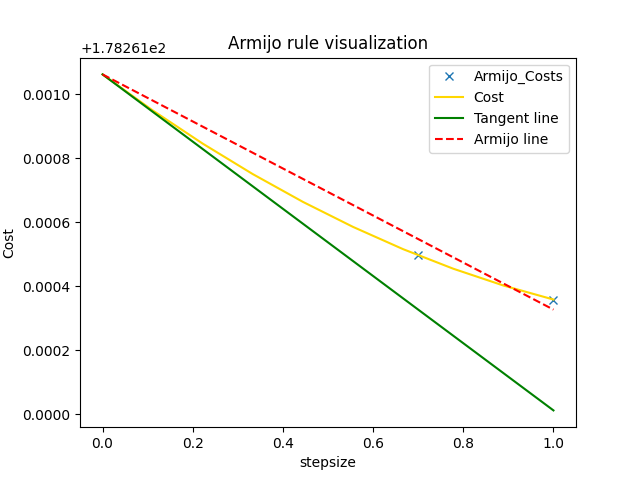
\includegraphics[width=1\textwidth]{pictures/arm_it_10.png}\hfill\\
  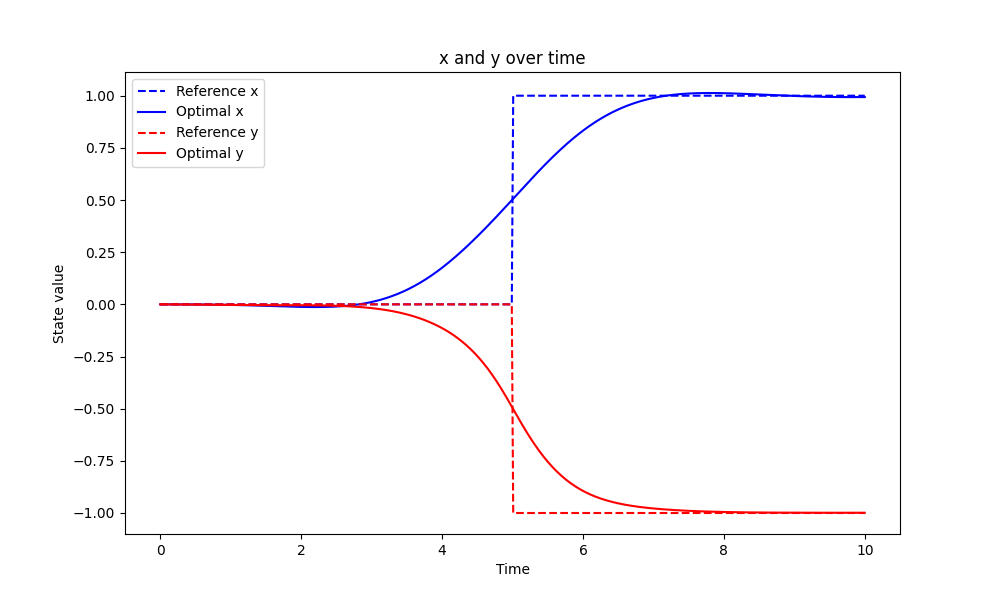
\includegraphics[width=1\textwidth]{pictures/new_it_10.png}\hfill
  \caption{Final iteration.}
\end{figure}

\subsection{Cost and Descent direction plot}
 Here the norm of the descent direction along iterations (in semi-logarithmic scale) and the cost along iterations (in semi-logarithmic scale) are shown: 
 
 \begin{figure}[h]
  \centering
  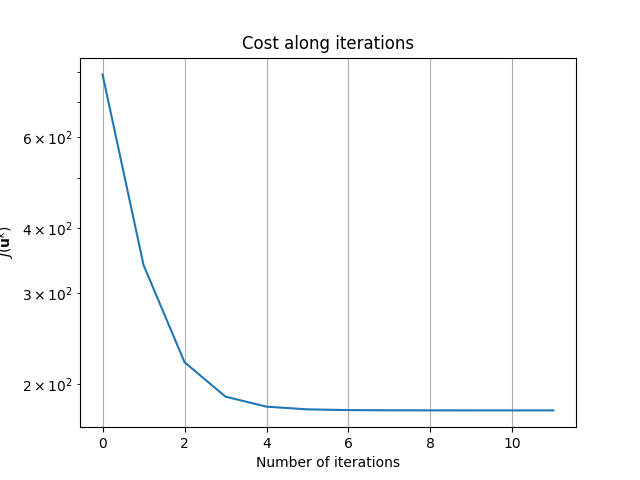
\includegraphics[width=1\textwidth]{pictures/cost_task1.png}\hfill \\
  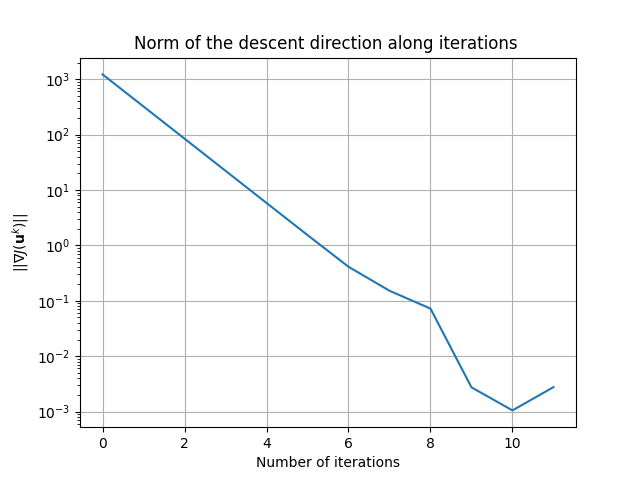
\includegraphics[width=1\textwidth]{pictures/descent_task1.png}\hfill
  \caption{Cost and descent direction norm.}
\end{figure}

\chapter{Task 2 - Trajectory generation (II)}
In task 2 we want to generate a desired (smooth) state$-$input curve and perform the trajectory generation task of Task 1 on this new desired trajectory.

In order to generate a smooth state-input curve we opted for a sigmoid trajectory that starts on the first equilibrium state and finishes on the second one.
The sigmoid function, often denoted as $\sigma(x)$, is defined as:
\[
\sigma(x) = \frac{1}{1 + e^{-x}}
\]
The Figure below illustrates the behavior of the sigmoid function.

\begin{figure}[h]
  \centering
  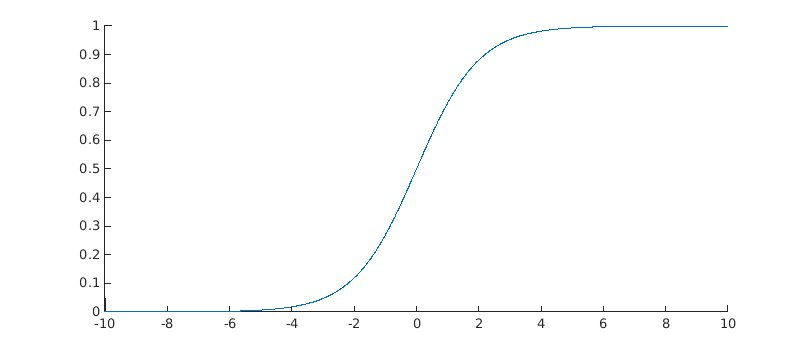
\includegraphics[width=0.6\textwidth]{pictures/sigmoide_graph.png}
  \caption{Behaviour of the sigmoid}
  \label{fig:sigmoid_plot}
\end{figure}

The choice of reference trajectory plays a crucial role in the performance and convergence characteristics of the Linear Quadratic Regulator (LQR) algorithm, it trapresents a more feasible reference for the trajectory.

The continuity of a smooth trajectory can facilitate the convergence of the LQR algorithm, as the system can gradually adapt to reference variations.

Furthermore, a smooth trajectory can help minimize the control energy required by the system. If the trajectory is already "close" to the optimal solution, the LQR algorithm may converge more quickly than in a situation where the reference has sharp changes.

\section{Results}
In this section, we present the outcomes of the Linear Quadratic Regulator on a sigmoid reference trajectory.

We applied this method to two different cases. In the first case, the equilibria are two distinct positions in space, and in the second case they are two distinct constant linear velocities. In the second case the trajectory for the state relative to the position x and y is obtained with the integration of the speed reference.

An example of the two cases follows:

\begin{figure}[H]
  \centering
  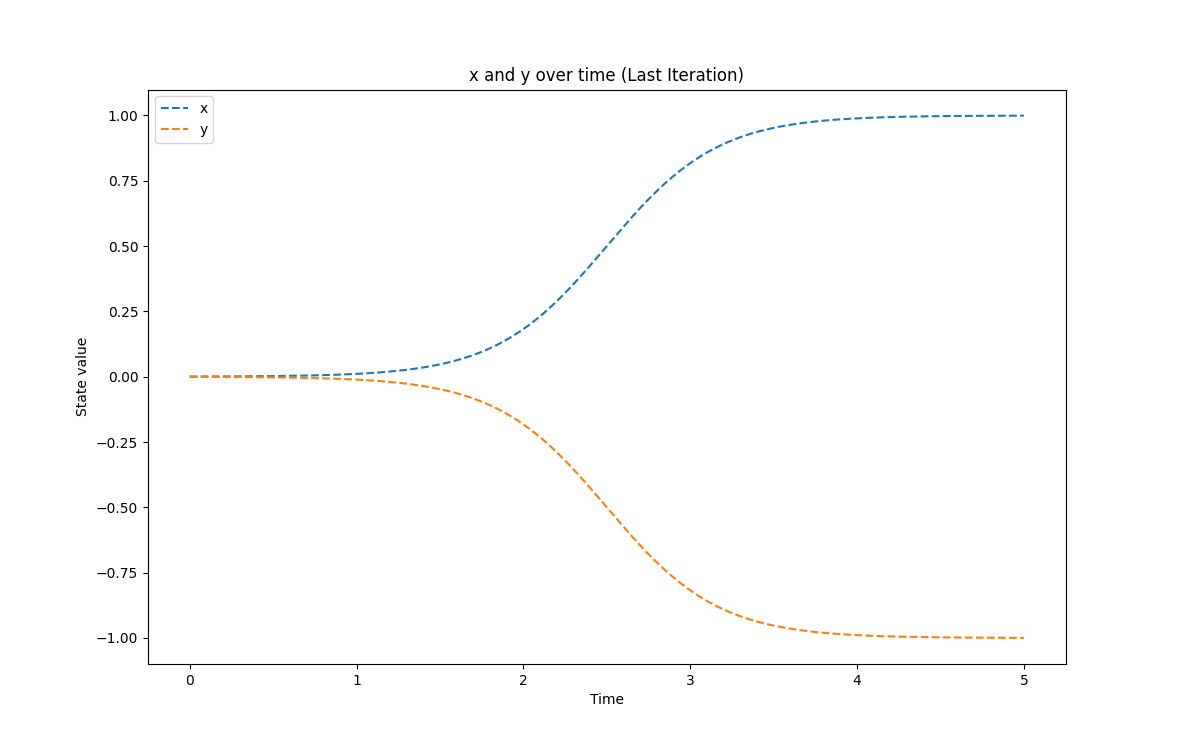
\includegraphics[width=0.6\textwidth]{pictures/Figure_1_posizione_smooth}\hfill
  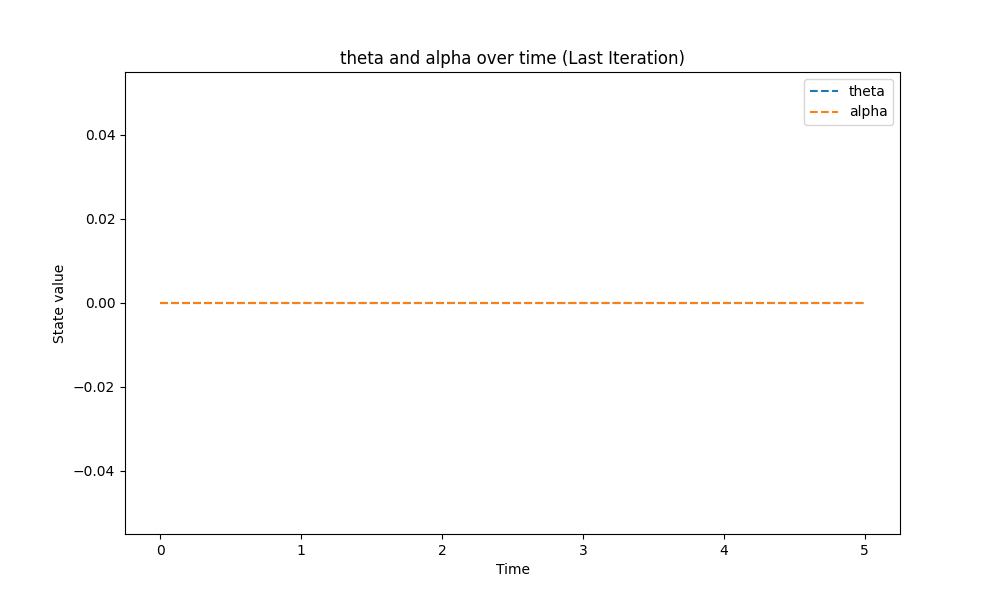
\includegraphics[width=0.6\textwidth]{pictures/Figure_2_posizione_smooth}\hfill
  \caption{Case 1: configuration reference over time.}
  \label{fig:Reference trajectory}
\end{figure}

\begin{figure}[H]
  \centering
  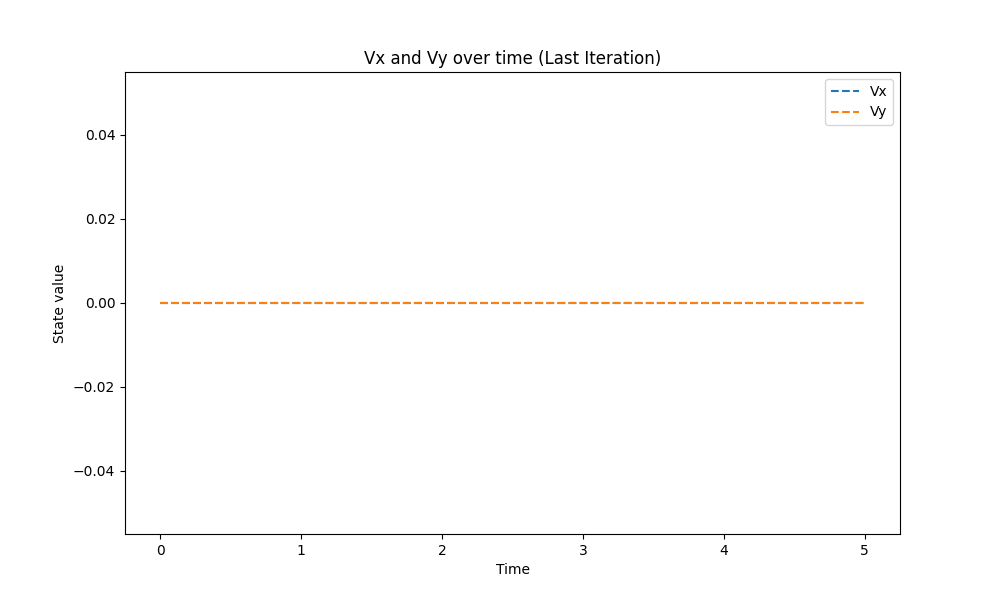
\includegraphics[width=0.85\textwidth]{pictures/Figure_3_posizione_smooth}\hfill \\
  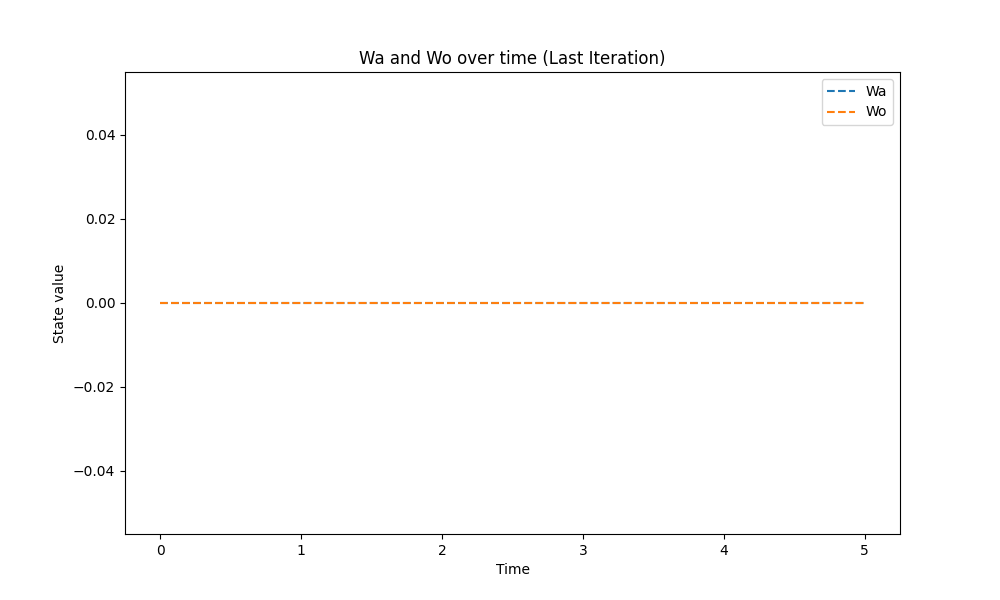
\includegraphics[width=0.85\textwidth]{pictures/Figure_4_posizione_smooth}\hfill
  \caption{Case 1: velocities reference over time.}
  \label{fig:Reference trajectory}
  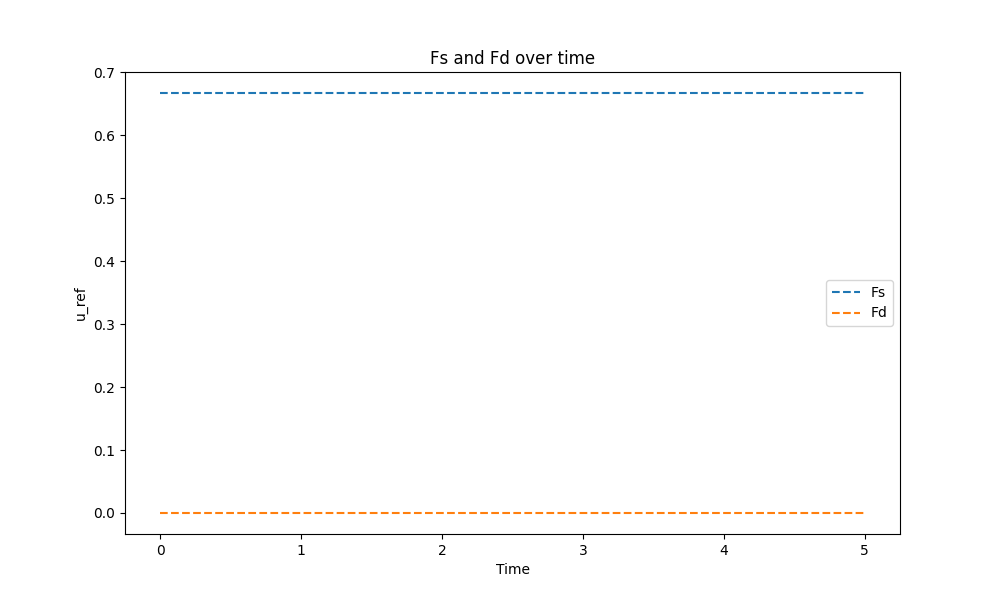
\includegraphics[width=0.85\textwidth]{pictures/Figure_5_posizione_smooth}
  \caption{Case 1: Input reference over time.}
  \label{fig:Reference trajectory}
\end{figure}

\begin{figure}[H]
  \centering
  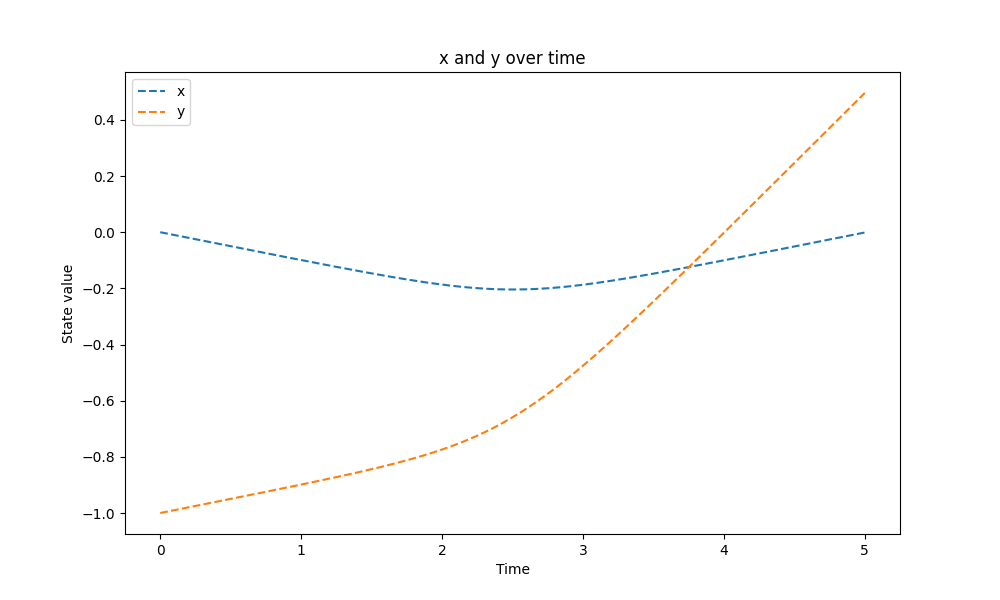
\includegraphics[width=0.9\textwidth]{pictures/Figure_1_velocita_smooth}\hfill\\
  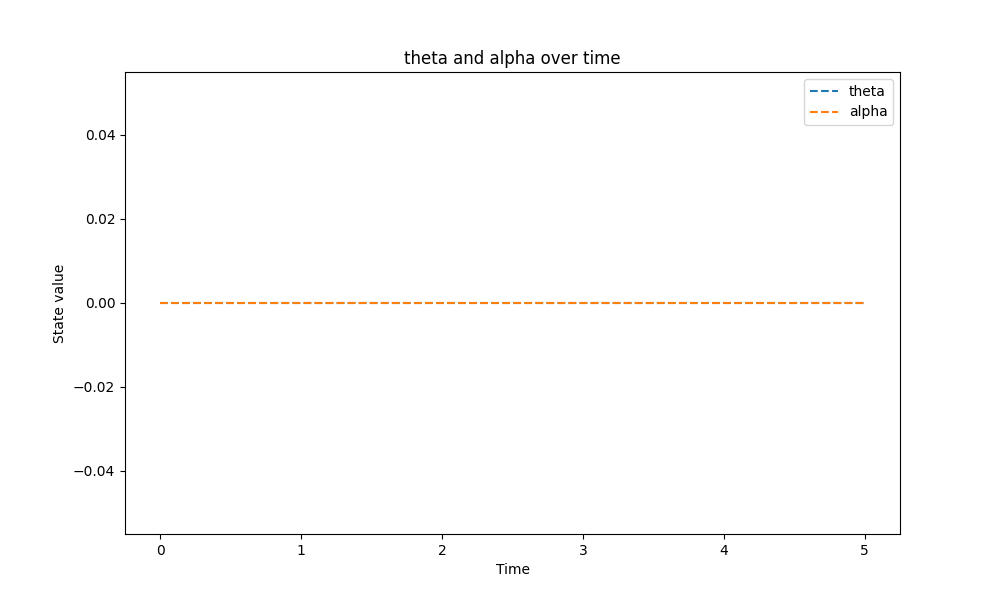
\includegraphics[width=0.9\textwidth]{pictures/Figure_2_velocita_smooth}\hfill
  \caption{Case 2: configuration reference over time.}
  \label{fig:Reference trajectory}
\end{figure}

\begin{figure}[H]
  \centering
  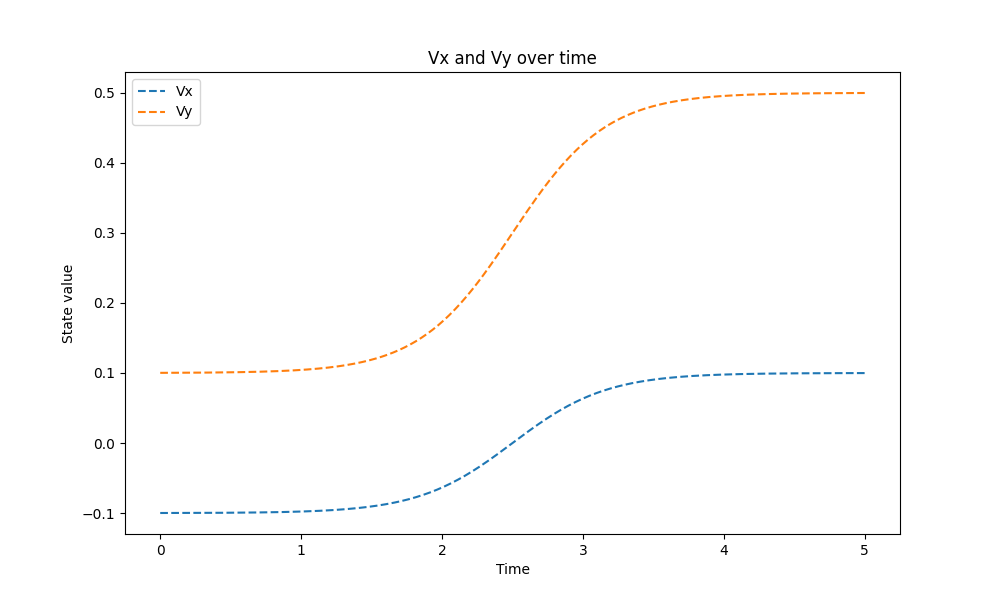
\includegraphics[width=0.85\textwidth]{pictures/Figure_3_velocita_smooth}\hfill \\
  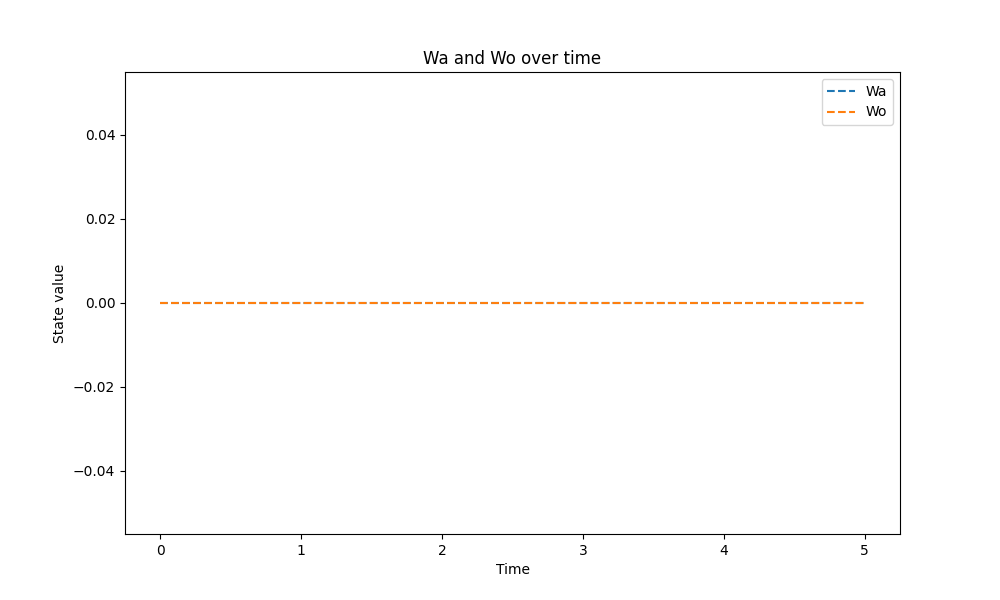
\includegraphics[width=0.85\textwidth]{pictures/Figure_4_velocita_smooth}\hfill
  \caption{Case 2: velocities reference over time.}
  \label{fig:Reference trajectory}
  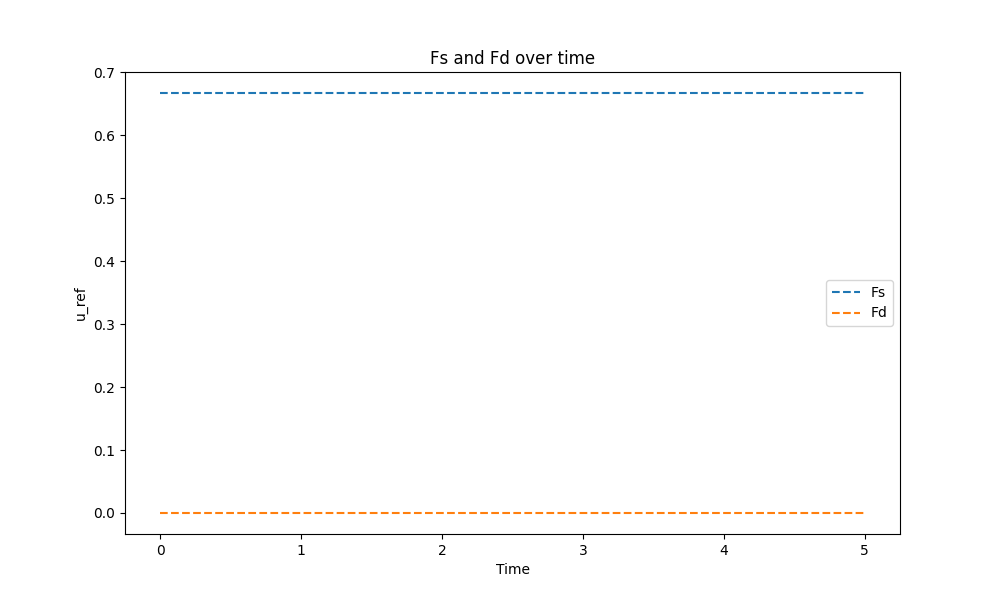
\includegraphics[width=0.85\textwidth]{pictures/Figure_5_velocita_smooth}
  \caption{Case 2: Input reference over time.}
  \label{fig:Reference trajectory}
\end{figure}

\subsection{Optimal trajectory}
In this section, we present the outcomes of the Linear Quadratic Regulator on the reference trajectory provided by equilibria that are two distinct positions in space (Case 1).

In the following pages the optimal trajectory found by our algorithm is shown.

\begin{figure}[H]
  \centering
  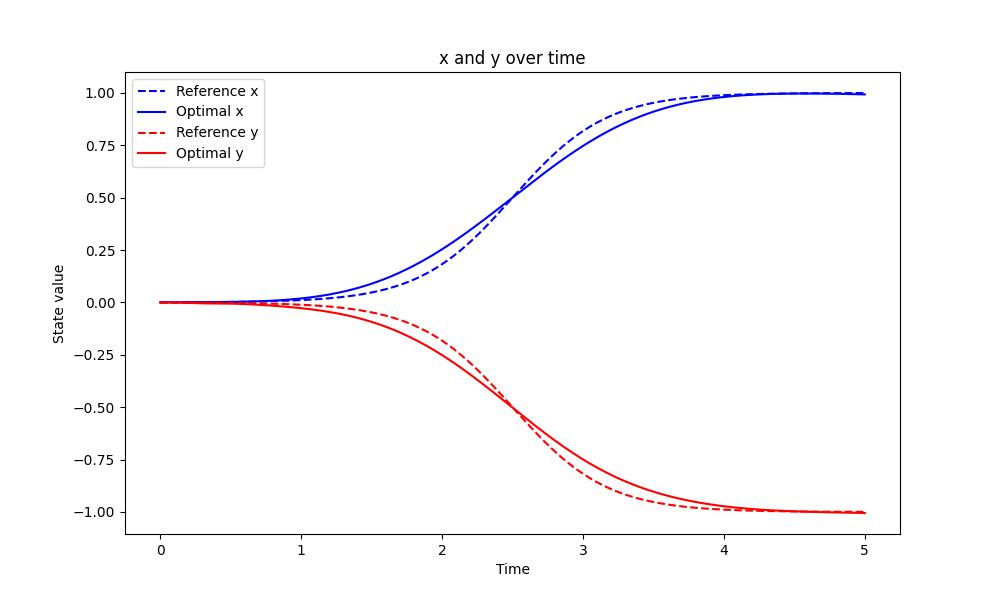
\includegraphics[width=0.9\textwidth]{pictures/Figure_1_opt_smooth.png}\hfill 
  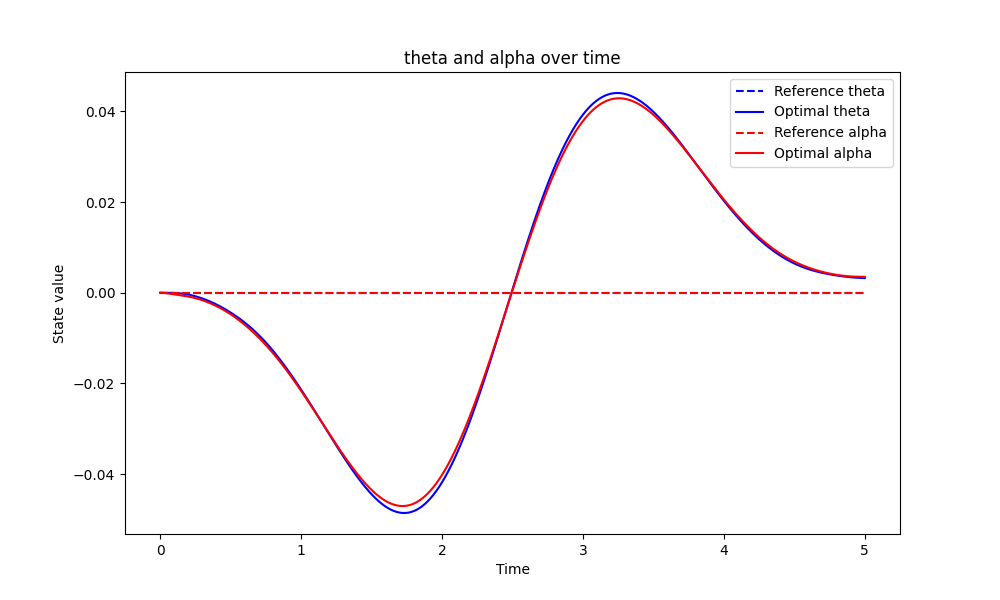
\includegraphics[width=0.9\textwidth]{pictures/Figure_2_opt_smooth.png}\hfill
  \caption{Optimal configuration over time.}
  \label{fig:Reference trajectory}
\end{figure}

\begin{figure}[H]
  \centering
  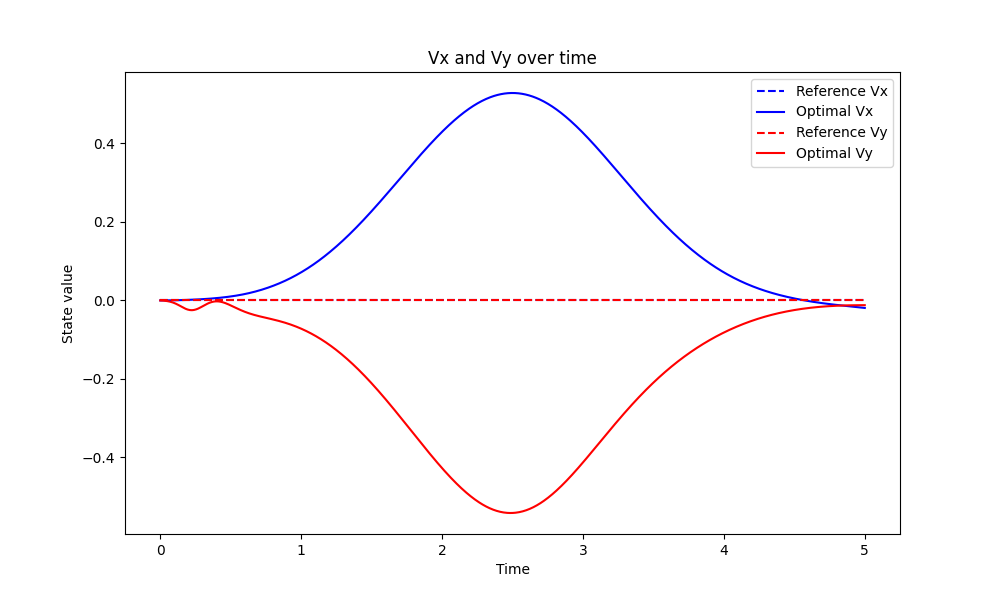
\includegraphics[width=0.85\textwidth]{pictures/Figure_3_opt_smooth.png}\hfill \\
  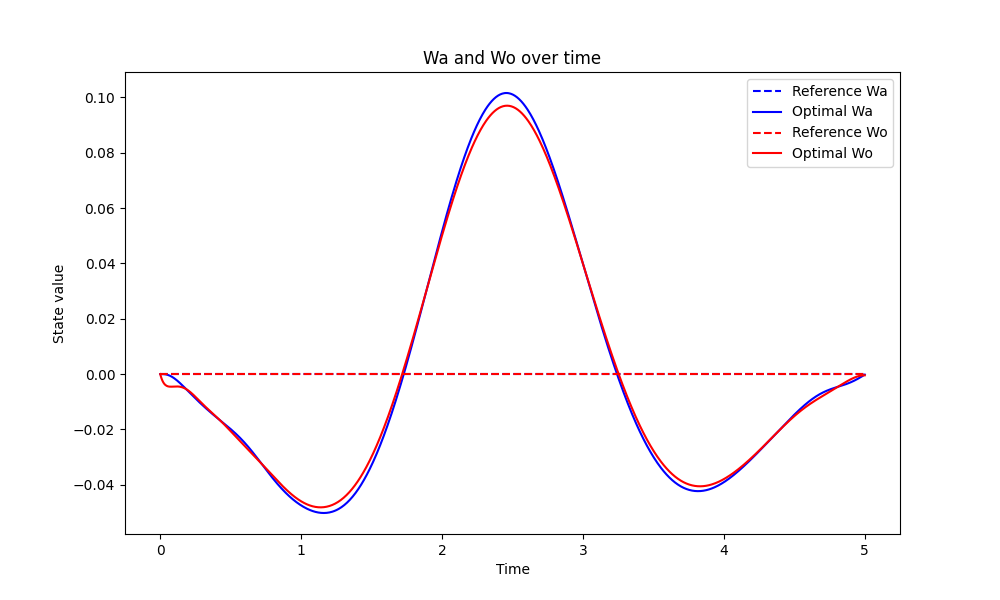
\includegraphics[width=0.85\textwidth]{pictures/Figure_4_opt_smooth.png}\hfill
  \caption{optimal velocities over time.}
  \label{fig:Reference trajectory}
  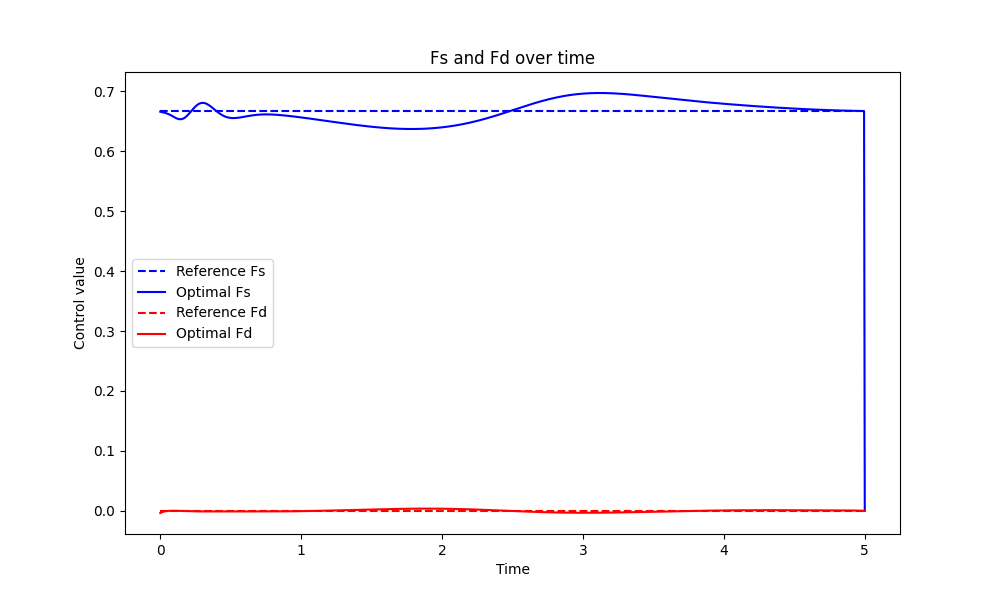
\includegraphics[width=0.85\textwidth]{pictures/Figure_5_opt_smooth.png}
  \caption{Optimal input over time.}
  \label{fig:Reference trajectory}
\end{figure}


\subsection{Suboptimal trajectories}
To illustrate the iterative evolution of the algorithm, we display only the x and y coordinates of the quadrotor over time and the armijos plot, providing an overview of the overall progression. Refer to the code for more details.
\begin{figure}[H]
  \centering
  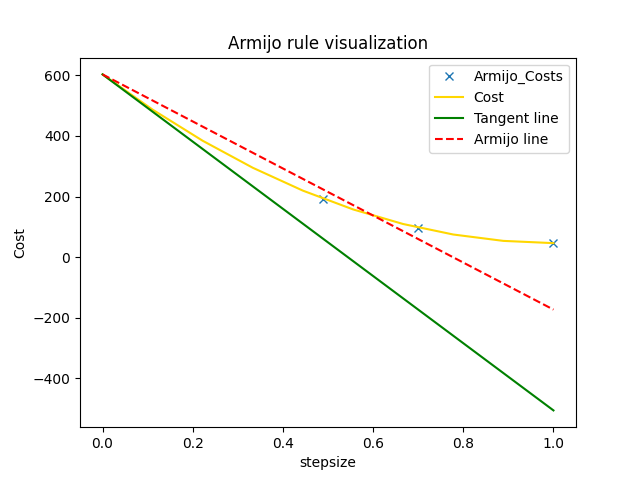
\includegraphics[width=1\textwidth]{pictures/Figure_1_1.png}\hfill \\
  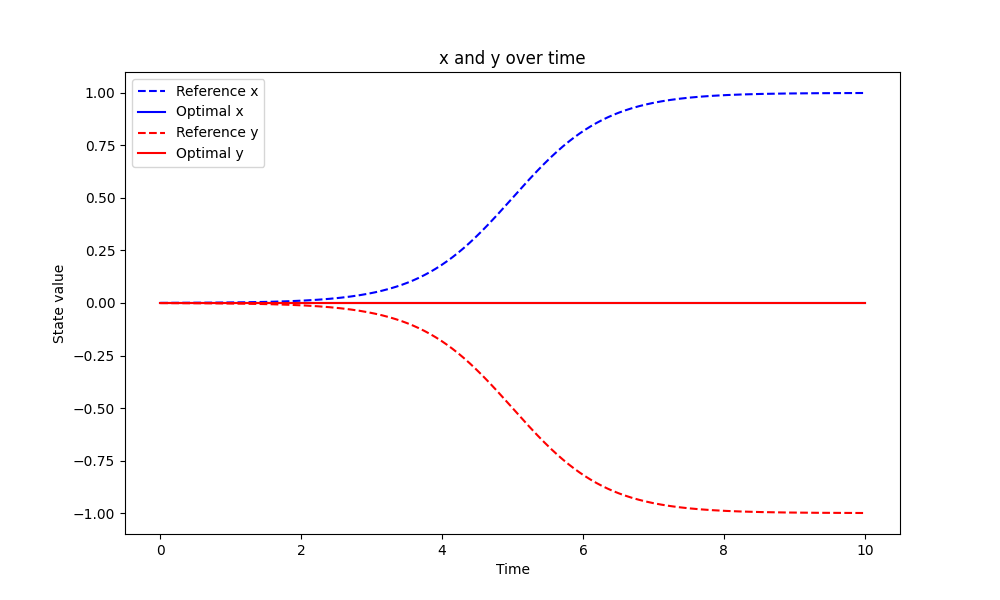
\includegraphics[width=1\textwidth]{pictures/Figure_1_2.png}\hfill
  \caption{First iteration.}
  \label{fig:Reference trajectory}
\end{figure}

\begin{figure}[H]
  \centering
  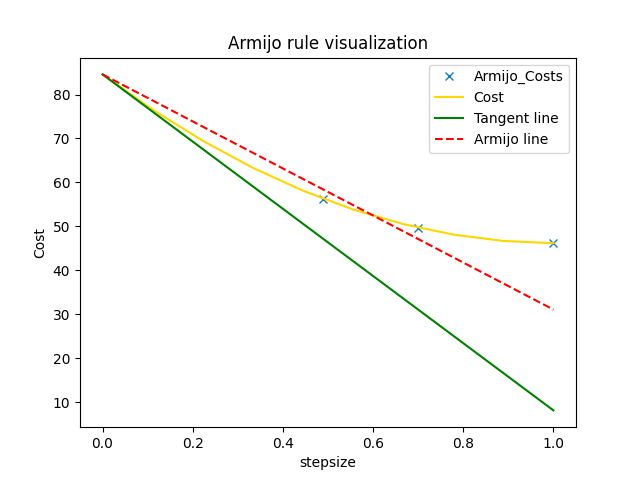
\includegraphics[width=1\textwidth]{pictures/Figure_2_1.png}\hfill \\
  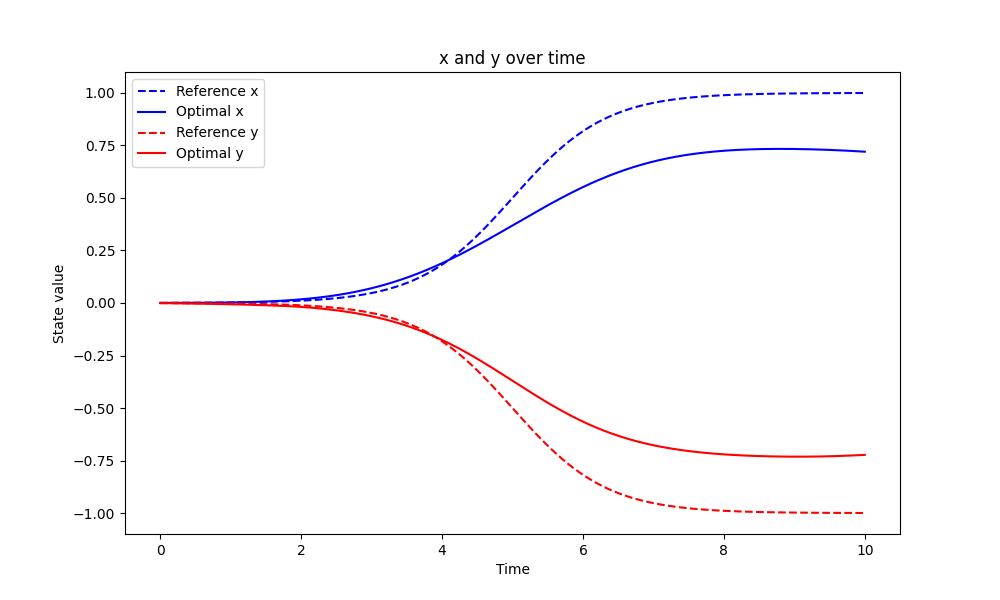
\includegraphics[width=1\textwidth]{pictures/Figure_2_2.png}\hfill
  \caption{Third iteration.}
  \label{fig:Reference trajectory}
\end{figure}

\begin{figure}[H]
  \centering
  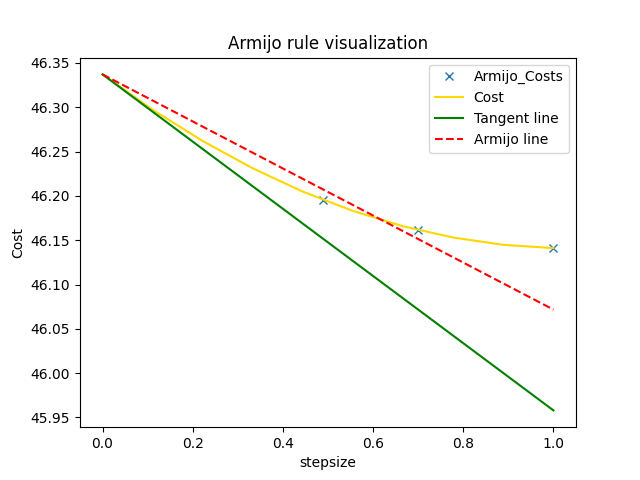
\includegraphics[width=1\textwidth]{pictures/Figure_3_1.png}\hfill\\
  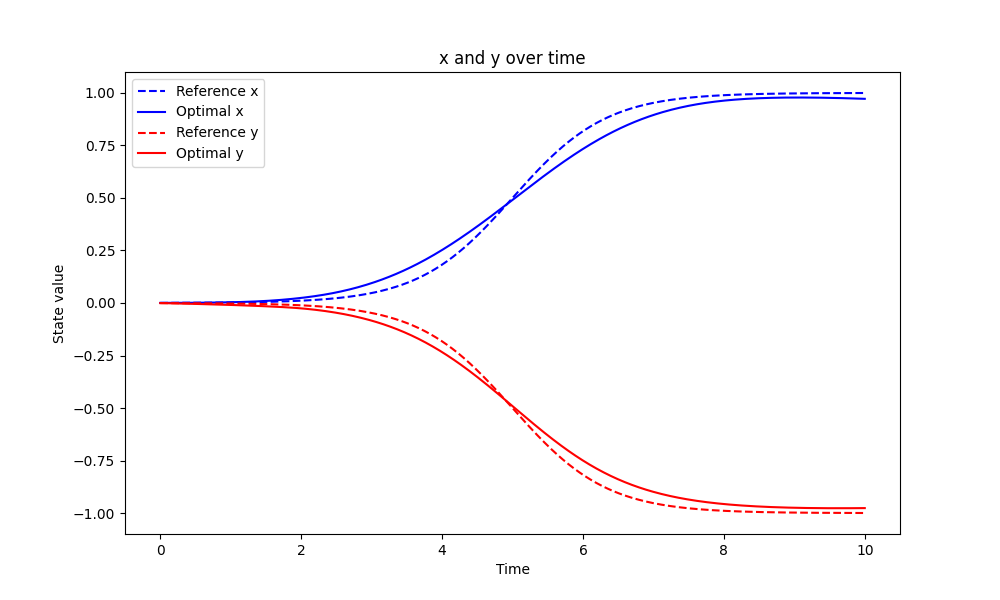
\includegraphics[width=1\textwidth]{pictures/Figure_3_2.png}\hfill
  \caption{Seventh iteration.}
  \label{fig:Reference trajectory}
\end{figure}

\begin{figure}[H]
  \centering
  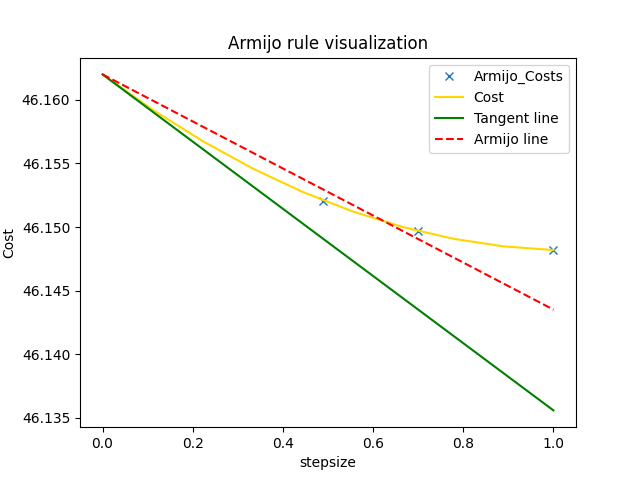
\includegraphics[width=1\textwidth]{pictures/Figure_4_1.png}\hfill\\
  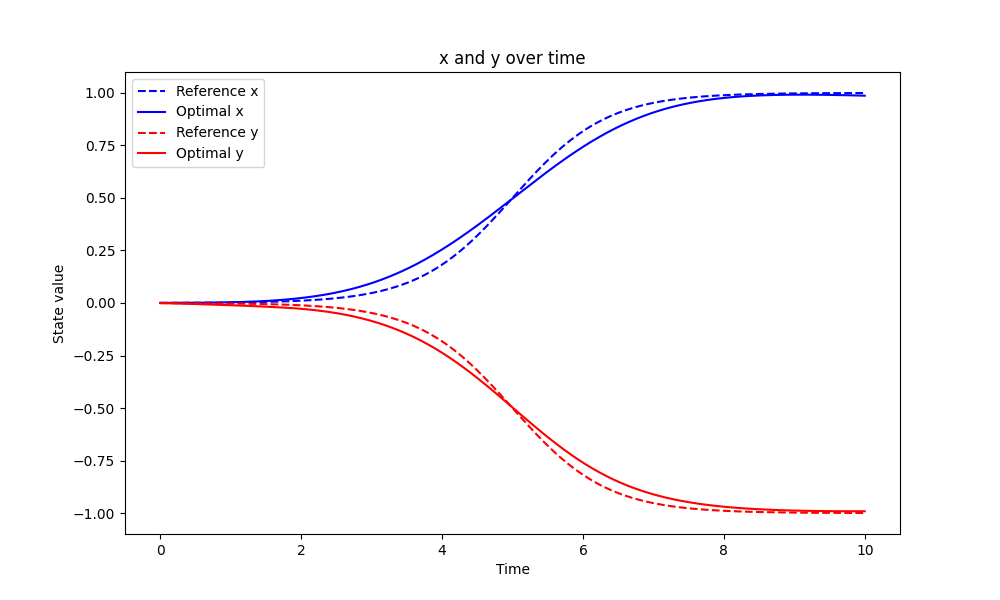
\includegraphics[width=1\textwidth]{pictures/Figure_4_2.png}\hfill
  \caption{Final iteration.}
\end{figure}

On the code you will also find the outcomes of the Linear Quadratic Regulator on the reference trajectory provided by equilibria that are two distinct velocity in space (Case 2).

\chapter{Task 3 - Trajectory tracking via LQR}
In task 3 we want to take the vehicle dynamics linearized about the (optimal) trajectory $(x_{opt}, u_{opt})$ computed in
Task 2 and then exploit the LQR algorithm to track this reference trajectory.

\section{Q and R definition}
Costs for closed loop Control:
\[
Q = \begin{bmatrix}
1 & 0 & 0 & 0 & 0 & 0 & 0 & 0 \\
0 & 1 & 0 & 0 & 0 & 0 & 0 & 0 \\
0 & 0 & 1 & 0 & 0 & 0 & 0 & 0 \\
0 & 0 & 0 & 1 & 0 & 0 & 0 & 0 \\
0 & 0 & 0 & 0 & 1 & 0 & 0 & 0 \\
0 & 0 & 0 & 0 & 0 & 1 & 0 & 0 \\
0 & 0 & 0 & 0 & 0 & 0 & 1 & 0 \\
0 & 0 & 0 & 0 & 0 & 0 & 0 & 1 \\
\end{bmatrix}
\]
\[
R = \begin{bmatrix}
3 & 0 \\
0 & 3 \\
\end{bmatrix}
\]

\section{Closed loop LQR}

\textbf{Evaluate the closed loop gain}\vspace{8pt} \\
Linearize the system dynamics evaluating 
\[\nabla_1 f_t(x_k^t, u_k^t), \nabla_2 f_t(x_k^t, u_k^t), \nabla_1 \ell_t(x_k^t, u_k^t), \nabla_2 \ell_t(x_k^t, u_k^t), \nabla \ell_T(x_k^T)\] 
Compute the closed loop gain $K_k^t$, for all $t = 0, \ldots, T - 1$:
\begin{align*}
\min_{\Delta x, \Delta u} &\sum_{t=0}^{T-1} \left( \nabla_1 \ell_t(x_k^t, u_k^t) \Delta x_t + \nabla_2 \ell_t(x_k^t, u_k^t) \Delta u_t \right)^\top \begin{bmatrix} \Delta x_t \\ \Delta u_t \end{bmatrix} \\
&+ \frac{1}{2} \begin{bmatrix} \Delta x_t \\ \Delta u_t \end{bmatrix}^\top \begin{bmatrix} Q_k^t & S_k^{t,\top} \\ S_k^t & R_k^t \end{bmatrix} \begin{bmatrix} \Delta x_t \\ \Delta u_t \end{bmatrix} \\
&+ \nabla \ell_T(x_k^T)^\top \Delta x_T + \frac{1}{2} \Delta x_T^\top Q_k^T \Delta x_T
\end{align*}
\textbf{Step 2: Compute new state-input trajectory}\vspace{8pt} \\
Implementing step-size selection rule, e.g., Armijo) \\
Forward integrate (closed-loop), for all  t = 0, \ldots, T - 1,  with  $x_{k+1,0} = x_{\text{init}}$ \vspace{8pt}\\
$u_{tracked,t} = u_k^t + K_k^t (x_{tracked,t} - x_{optimal,t})$\\
$x_{tracked,t+1} = f_t(x_{tracked,t}, u_{tracked,t})$\\


\subsection{Plots}
In order to evaluate the tracking performance of the controller, the initial position of the quadrotor is set to be different from that of the optimal trajectory. Examples of the tracking performance are shown in the following plots.

\begin{figure}[H]
  \centering
  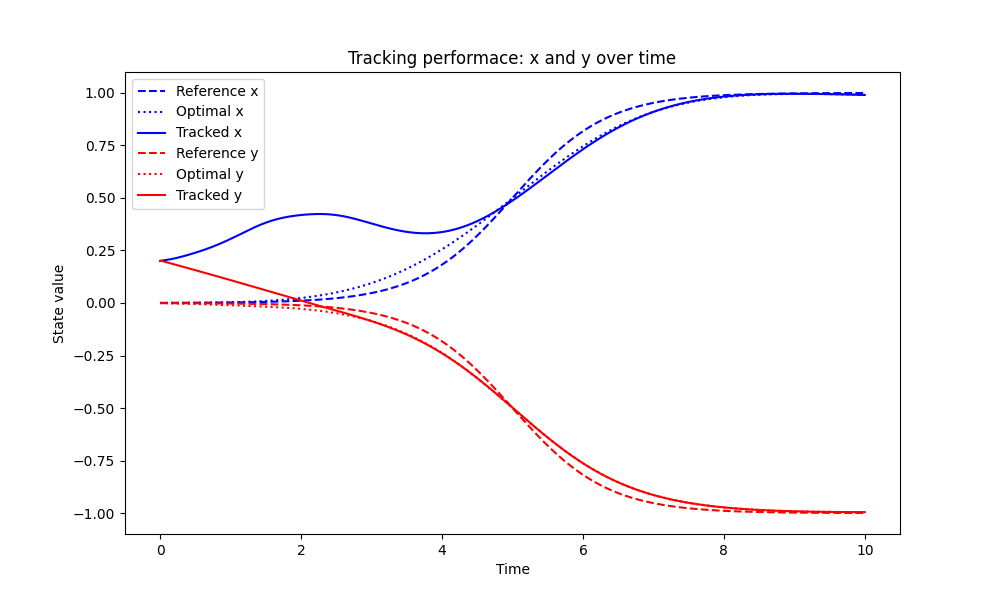
\includegraphics[width=1\textwidth]{pictures/tracking_xy.png}\hfill \\
  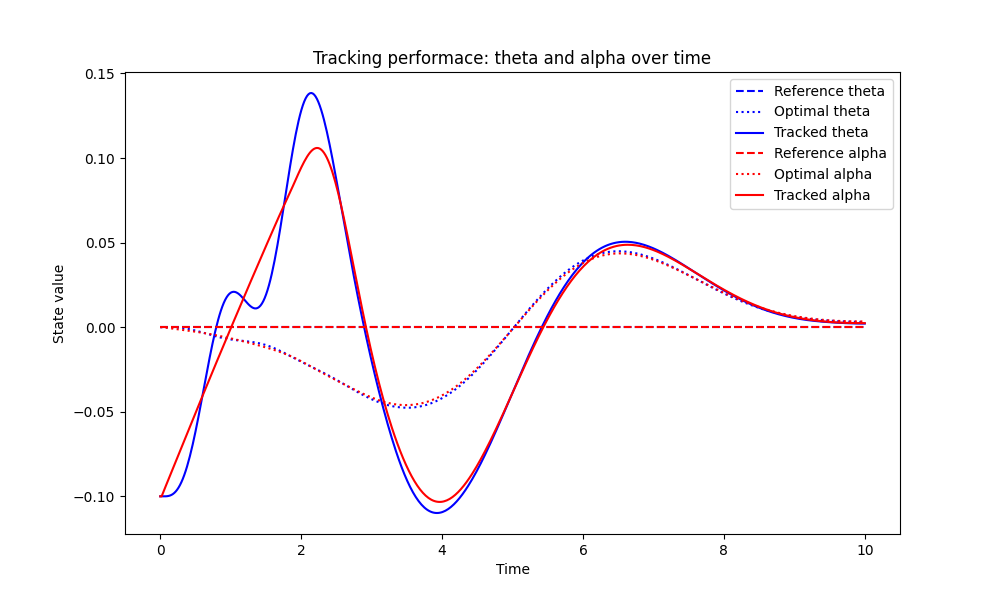
\includegraphics[width=1\textwidth]{pictures/tracking_theta_alpha.png}\hfill
  \caption{configuration tracking.}
  \label{fig:Reference trajectory}
\end{figure}

\begin{figure}[H]
  \centering
  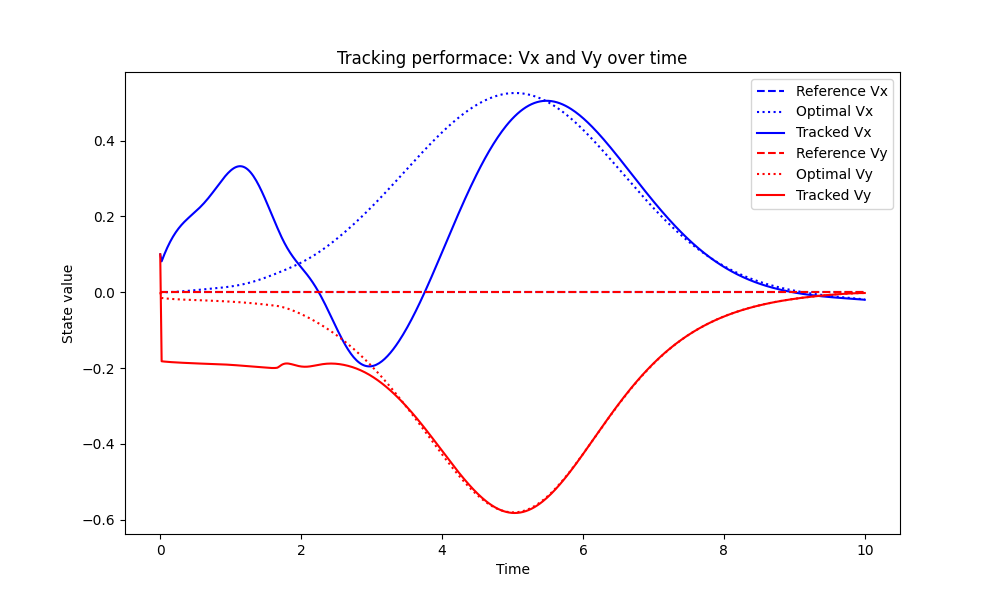
\includegraphics[width=1\textwidth]{pictures/tracking_vx_vy.png}\hfill \\
  \includegraphics[width=1\textwidth]{pictures/tracking_omega.png}\hfill
  \caption{velocity tracking.}
  \label{fig:Reference trajectory}
\end{figure}

\begin{figure}[H]
  \centering
  \includegraphics[width=1\textwidth]{pictures/tracking_input.png}\hfill \\
  \caption{input tracking.}
  \label{fig:Reference trajectory}
\end{figure}


\chapter{Task 4 - Trajectory tracking via MPC}
In task 4 we want to take the vehicle dynamics linearized about the (optimal) trajectory $(x_{opt}, u_{opt})$ computed in
Task 2 and then exploit an MPC algorithm to track this reference trajectory.

\section{Model Predictive Control}

The goal of Model predictive Control (MPC) is to control a system via a stabilizing controller that minimizes a certain cost function, enforces some constraint for all t and works online. This is implemented by solving an optimal control problem at each sampling time and applying the first optimal input: 

For each t: 
\begin{itemize}
    \item Measure the current state $x_t$
    \item Compute the optimal trajectory $x^{*}_{t|t},..., x^{*}_{t+T|t}, u^{*}_{t|t}, ..., u^{*}_{t+T-1|t}$ with initial condition $x_t$
    \item Apply the first control input $u^{*}_{t|t}$
    \item Measure $x_{t+1}$ and repeat
\end{itemize}

\begin{figure}[htp]
\centering
\includegraphics[width=0.5\textwidth]{pictures/MPC}
\caption{Model Predictive Control}
\label{fig:MPC}
\end{figure}


\subsection{The optimal control problem to be solved at each t}

At each time instant we want to solve

\begin{align*}
\min_{\substack{x_t,...,x_{t+T} \\ u_t,...,u_{t+T-1}}} &\sum_{\tau=t}^{t+T-1} l_\tau (x_\tau, u_\tau) + l_{t+T}(x_{t+T})
\end{align*}

\begin{align*} subject \quad to \qquad 
 x_{\tau+1} = f(x_\tau, u_\tau) \qquad \forall \tau = t, ..., t+T-1 \\ 
 x_{\tau} \in \textit{X}, u_{\tau} \in \textit{U} \qquad \forall \tau = t, ..., t+T \qquad\\
 x_t = x^{meas}_t \qquad \qquad \qquad \qquad \qquad \qquad 
\end{align*}

where 
\begin{itemize}
    \item $x_{\tau + 1} = f(x_\tau, u_\tau)$ is the so-called prediction model
    \item $x^{meas}_t$ is the state (of the real system) measured at t
\end{itemize}

\subsection{The Linear Quadratic Case}

In our case, the dynamics is linear because we linearized it about the optimal trajectory $(x_{opt}, u_{opt})$ computed in task 2. Therefore we can consider the MPC case where the dynamics is linear and the cost quadratic: 

At each time t with initial measured state $x_t^{meas}$ we want to solve the LQ problem 

\begin{align*}
\min_{\substack{x_t,...,x_{t+T} \\ u_t,...,u_{t+T-1}}} &\sum_{\tau=t}^{t+T-1} x_\tau^T Q_\tau x_\tau + u_\tau^T R_\tau u_\tau + x_{t+T}^T Q_T x_{t+T}
\end{align*}

\begin{align*} subject \quad to \qquad 
 x_{\tau+1} = A_\tau x_\tau + B_\tau u_\tau \qquad \forall \tau = t, ..., t+T-1 \\ 
 x_t = x^{meas}_t \qquad \qquad \qquad \qquad \qquad \qquad \qquad \quad 
\end{align*}

where  
\begin{itemize}
    \item T is the prediction horizon
    \item $x_{\tau} \in \mathbb{R}^n$ and $u_{\tau} \in \mathbb{R}^m$
    \item $A_{\tau} \in \mathbb{R}^{nxn}$ and $B_{\tau} \in \mathbb{R}^{nxm}$ is the prediction model 
    \item $Q_{\tau} \in \mathbb{R}^{nxn}$ and $Q_{\tau} = Q_{\tau}^T \geq 0 \forall \tau$  
    \item $R_{\tau} \in \mathbb{R}^{mxm}$ and $R_{\tau} = R_{\tau}^T > 0 \forall \tau$ 
    \item $Q_{T} \in \mathbb{R}^{nxn}$ and $Q_{T} = Q_{T}^T \geq 0 $ 
    
\end{itemize}

\section{Tracking of $(x_{opt}, u_{opt})$}
Since we want to track the optimal trajectory throught Model Predictive Control, the cost function that we are interested in minimizing is the one in which $x_\tau$ and $u_\tau$ are the errors between the predicted trajectory ($x^{mpc}$, $u^{mpc}$) and the optimal one ($x^{opt}$, $u^{opt}$): 

\[x_\tau = x_\tau^{mpc} - x_\tau^{opt}\]
\[u_\tau = u_\tau^{mpc} - u_\tau^{opt}\]

Therefore, the LQ problem we are solving at each t results: 

\[\min_{\substack{x_t,...,x_{t+T} \\ u_t,...,u_{t+T-1}}} \quad \sum_{\tau=t}^{t+T-1} (x_\tau^{mpc} - x_\tau^{opt})^T Q_\tau (x_\tau^{mpc} - x_\tau^{opt}) +\]
\[\qquad \qquad + (u_\tau^{mpc} - u_\tau^{opt})^T R_\tau (u_\tau^{mpc} - u_\tau^{opt}) + \]
\[\qquad \qquad + (x_{t+T}^{mpc} - x_{t+T}^{opt})^T Q_T (x_{t+T}^{mpc} - x_{t+T}^{opt}) \]

\begin{align*} subject \quad to \quad 
 x_{\tau+1}^{mpc} - x_{\tau+1}^{opt} = A_\tau (x_\tau^{mpc} - x_\tau^{opt}) + B_\tau  (u_\tau^{mpc} - u_\tau^{opt}) \quad \\
 \forall \tau = t, ..., t+T-1 \\ 
 x_t^{mpc} - x_t^{opt} = x^{meas}_t  - x_t^{opt}\qquad \qquad \qquad \qquad \qquad \quad 
\end{align*}


Our simulation horizon is of 500 samples, and we choose the MPC prediction horizon to be of 100 samples, which allows the system to exhibit satisfactory control performance, meet the desired objectives, and remain computationally feasible. 

Regarding the costs, oure choiche is based on trial and error in order to guarantee some settling time and overshoot and it is the following: 

\[
QQ_\tau = \begin{bmatrix}
9 & 0 & 0 & 0 & 0 & 0 & 0 & 0 \\
0 & 9 & 0 & 0 & 0 & 0 & 0 & 0 \\
0 & 0 & 1 & 0 & 0 & 0 & 0 & 0 \\
0 & 0 & 0 & 1 & 0 & 0 & 0 & 0 \\
0 & 0 & 0 & 0 & 1 & 0 & 0 & 0 \\
0 & 0 & 0 & 0 & 0 & 1 & 0 & 0 \\
0 & 0 & 0 & 0 & 0 & 0 & 5 & 0 \\
0 & 0 & 0 & 0 & 0 & 0 & 0 & 5 \\
\end{bmatrix}
\]
\[
RR_\tau = \begin{bmatrix}
3 & 0 \\
0 & 3 \\
\end{bmatrix}
\]
\[
QQ_T = QQ_\tau
\]

\section{Results}

To showcase the tracking performances, we consider a perturbed initial condition (different than $x_{opt, 0}$): 

\[ \textbf{x}_0 = \begin{bmatrix} x_{p,0} \\ y_{p,0} \\ \alpha_0 \\ \theta_0 \\ v_{x,0} \\ v_{y,0} \\ \omega_{\alpha,0} \\ \omega_{\theta,0} \end{bmatrix} = \begin{bmatrix}   0.4 \\ 0.4 \\ -0.1 \\ -0.1 \\ 0.1 \\ 0.1 \\ 0 \\ 0 \end{bmatrix} \]


\subsection{System trajectory and desired optimal trajectory}
Below, the plots of the MPC trajectory tracking the desired optimal trajectory (denoted as LQR) for the single states and inputs: 

\begin{figure}[H]
\centering
\includegraphics[width=0.9\textwidth]{pictures/mpc1.png}
\caption{$x_1$}
\label{fig:mpc1}
\end{figure}

\begin{figure}[H]
\centering
\includegraphics[width=0.9\textwidth]{pictures/mpc2.png}
\caption{$x_2$}
\label{fig:mpc2}
\end{figure}

\begin{figure}[H]
\centering
\includegraphics[width=0.9\textwidth]{pictures/mpc3.png}
\caption{$x_3$}
\label{fig:mpc3}
\end{figure}

\begin{figure}[H]
\centering
\includegraphics[width=0.9\textwidth]{pictures/mpc4.png}
\caption{$x_4$}
\label{fig:mpc4}
\end{figure}

\begin{figure}[H]
\centering
\includegraphics[width=0.9\textwidth]{pictures/mpc5.png}
\caption{$x_5$}
\label{fig:mpc5}
\end{figure}

\begin{figure}[H]
\centering
\includegraphics[width=0.9\textwidth]{pictures/mpc6.png}
\caption{$x_6$}
\label{fig:mpc6}
\end{figure}

\begin{figure}[H]
\centering
\includegraphics[width=0.9\textwidth]{pictures/mpc7.png}
\caption{$x_7$}
\label{fig:mpc7}
\end{figure}

\begin{figure}[H]
\centering
\includegraphics[width=0.9\textwidth]{pictures/mpc8.png}
\caption{$8_1$}
\label{fig:mpc8}
\end{figure}

\begin{figure}[H]
\centering
\includegraphics[width=0.9\textwidth]{pictures/mpc9.png}
\caption{$u_1$}
\label{fig:mpc9}
\end{figure}

\begin{figure}[H]
\centering
\includegraphics[width=0.9\textwidth]{pictures/mpc10.png}
\caption{$u_2$}
\label{fig:mpc10}
\end{figure}
 
\subsection{Tracking error for different initial conditions}

Given the perturbed initial condition \[ x_0 = [0.4, 0.4, -0.1, -0.1, 0.1, 0.1, 0, 0]^T\]
the following are the plots of the tracking error for single states and inputs: 


\begin{figure}[H]
\centering
\includegraphics[width=0.83\textwidth]{pictures/mpc11.png}
\caption{Tracking error for $x_1$}
\label{fig:mpc11}
\end{figure}

\begin{figure}[H]
\centering
\includegraphics[width=0.9\textwidth]{pictures/mpc12.png}
\caption{Tracking error for $x_2$}
\label{fig:mpc12}
\end{figure}

\begin{figure}[H]
\centering
\includegraphics[width=0.9\textwidth]{pictures/mpc13.png}
\caption{Tracking error for $x_3$}
\label{fig:mpc13}
\end{figure}

\begin{figure}[H]
\centering
\includegraphics[width=0.9\textwidth]{pictures/mpc14.png}
\caption{Tracking error for $x_4$}
\label{fig:mpc14}
\end{figure}

\begin{figure}[H]
\centering
\includegraphics[width=0.9\textwidth]{pictures/mpc15.png}
\caption{Tracking error for $x_5$}
\label{fig:mpc15}
\end{figure}

\begin{figure}[H]
\centering
\includegraphics[width=0.9\textwidth]{pictures/mpc16.png}
\caption{Tracking error for $x_6$}
\label{fig:mpc16}
\end{figure}

\begin{figure}[H]
\centering
\includegraphics[width=0.9\textwidth]{pictures/mpc17.png}
\caption{Tracking error for $x_7$}
\label{fig:mpc17}
\end{figure}

\begin{figure}[H]
\centering
\includegraphics[width=0.9\textwidth]{pictures/mpc18.png}
\caption{Tracking error for $x_8$}
\label{fig:mpc18}
\end{figure}

\begin{figure}[H]
\centering
\includegraphics[width=0.9\textwidth]{pictures/mpc19.png}
\caption{Tracking error for $u_1$}
\label{fig:mpc19}
\end{figure}

\begin{figure}[H]
\centering
\includegraphics[width=0.9\textwidth]{pictures/mpc20.png}
\caption{Tracking error for $u_2$}
\label{fig:mpc20}
\end{figure}

\chapter{Task 5 - Animation}
As required, we have implemented a simple animation, that starts automatically at the end of execution of Task 3. 

Below, some frames of the animation showing the movement of the quadrotor along the computed optimal trajectory starting from a perturbed initial condition (see task 3): 

\begin{figure}[H]
\centering
\includegraphics[width=0.9\textwidth]{pictures/ani0.png}
\caption{$t = 0s$}
\label{fig:ani1}
\end{figure}

\begin{figure}[H]
\centering
\includegraphics[width=0.9\textwidth]{pictures/ani05.png}
\caption{$t = 0.5s$}
\label{fig:ani05}
\end{figure}

\begin{figure}[H]
\centering
\includegraphics[width=0.9\textwidth]{pictures/ani11.png}
\caption{$t = 1.1s$}
\label{fig:ani11}
\end{figure}

\begin{figure}[H]
\centering
\includegraphics[width=0.9\textwidth]{pictures/ani17.png}
\caption{$t = 1.7s$}
\label{fig:ani17}
\end{figure}

\begin{figure}[H]
\centering
\includegraphics[width=0.9\textwidth]{pictures/ani24.png}
\caption{$t = 2.4s$}
\label{fig:ani24}
\end{figure}

\begin{figure}[H]
\centering
\includegraphics[width=0.9\textwidth]{pictures/ani49.png}
\caption{$t = 4.9s$}
\label{fig:ani49}
\end{figure}


%%%%%%%%%% Conclusions %%%%%%%%%%
\chapter*{Conclusions}
\addcontentsline{toc}{chapter}{Conclusions}

With the realization of this project we solved different tasks and were able to design an optimal control for a planar quadrotor with suspended load.

\begin{itemize}
    \item In the first task, a Newton's like algorithm was implemented to design the
optimal trajectoy allowing to follow a step reference to move from one equilibrium configuration to another. In order to do this, the Armijo algorithm for step size selection was exploited.
    \item In the second task we exploited again the Newton's like algorithm to design an optimal
trajectory between two equilibria, but with a reference curve designed as a sigmoid function.
    \item In the third task we used the LQR method to follow the optimal trajectory
designed in task 2. Furthermore, we proved that the controller is able
to achieve the target starting with perturbed initial conditions.
    \item In the fourth task we applied the MPC algorithm to track the
optimal trajectory designed in task 2 and we proved again that the controller is able to achieve the target starting with perturbed initial conditions.

\end{itemize}

%%%%%%%%%% Bibliography %%%%%%%%%%%
%\bibliography{bibfile}{}
%\bibliographystyle{plain}
%\addcontentsline{toc}{chapter}{Bibliography}


%%%%%%%%%%%%%%%%%%%%%%%%%%%%%%%%%%%%%%

\end{document}